\documentclass[11pt,a4paper]{article}
\usepackage[T1]{fontenc}
\usepackage[utf8]{inputenc}
\usepackage{fix-cm}
\usepackage[scaled=0.96]{helvet}
\renewcommand{\familydefault}{\sfdefault}
\usepackage{amsmath,amssymb,mathtools}
\usepackage{newtxmath}
\usepackage{bm}
\usepackage[margin=20mm,top=35mm,bottom=20mm,headheight=57pt,headsep=10mm]{geometry}
\usepackage{microtype,booktabs,array,tabularx,longtable,enumitem,needspace}
\usepackage[most]{tcolorbox}
\usepackage{fancyhdr,lastpage,xcolor}
\usepackage[hidelinks,pdfencoding=auto,psdextra]{hyperref}
\hypersetup{pdfauthor={MB1 research teaching edition},pdftitle={A Two-Cycle Quantum Conveyor - Questions (public example)},pdfsubject={APhO-style guided research exercise; not an official APhO examination},pdfkeywords={fractional Thouless pump, geometry, local error, questions}}
\definecolor{ink}{HTML}{172A3A}
\definecolor{sourcegreen}{HTML}{1B6B4B}
\definecolor{sourcewash}{HTML}{F4FAF6}
\definecolor{openred}{HTML}{A42B32}
\definecolor{openwash}{HTML}{FFF6F6}
\definecolor{rulegray}{HTML}{5E6670}
\setlength{\parindent}{0pt}
\setlength{\parskip}{5.4pt}
\setlength{\tabcolsep}{5pt}
\renewcommand{\arraystretch}{1.16}
\setlength{\emergencystretch}{2em}
\setlength{\abovedisplayskip}{7pt}
\setlength{\belowdisplayskip}{7pt}
\raggedbottom
\pagestyle{fancy}
\fancyhf{}
\fancyhead[L]{\begin{minipage}[b]{0.73\textwidth}\textbf{\large Theoretical Question Paper}\\[-1pt]{\small APhO-style research exercise \enspace|\enspace public example}\\[-1pt]{\footnotesize English --- public example}\end{minipage}}
\fancyhead[R]{\fontsize{29}{31}\selectfont\bfseries Q1-\thepage}
\renewcommand{\headrulewidth}{0.9pt}
\fancyfoot[L]{\footnotesize Not an official APhO paper \enspace\textbullet\enspace Advanced undergraduate level}
\fancyfoot[R]{\footnotesize \thepage/\pageref*{LastPage}}
\renewcommand{\footrulewidth}{0pt}
\newcommand{\ket}[1]{\lvert #1\rangle}
\newcommand{\bra}[1]{\langle #1\rvert}
\newcommand{\braket}[2]{\langle #1\vert #2\rangle}
\newcommand{\Tr}{\operatorname{Tr}}
\newcommand{\dd}{\mathrm d}
\newcommand{\hc}{\mathrm{h.c.}}
\newcommand{\norm}[1]{\left\lVert #1\right\rVert}
\newcommand{\Qbar}{\overline Q}
\newcommand{\parttitle}[3]{\par\vspace{2pt}{\large\bfseries\color{ink}Part #1. #2\hfill\normalsize(#3 points)}\par\vspace{4pt}}
\newcommand{\pagetitle}[1]{{\large\bfseries\color{ink}#1}\par\vspace{4pt}}
\newtcolorbox{greenbox}[1]{enhanced,breakable,colback=sourcewash,colframe=sourcegreen,boxrule=0.9pt,arc=0pt,left=8pt,right=8pt,top=6pt,bottom=6pt,before skip=7pt,after skip=8pt,title={\strut AVAILABLE --- #1},colbacktitle=sourcewash,coltitle=sourcegreen,fonttitle=\bfseries\small,titlerule=0pt,fontupper=\small}
\newtcolorbox{redbox}[1]{enhanced,breakable,colback=openwash,colframe=openred,boxrule=0.9pt,arc=0pt,left=8pt,right=8pt,top=6pt,bottom=6pt,before skip=7pt,after skip=8pt,title={\strut NOT ESTABLISHED FOR MB1 --- #1},colbacktitle=openwash,coltitle=openred,fonttitle=\bfseries\small,titlerule=0pt,fontupper=\small}
\newcommand{\question}[3]{\begin{tcolorbox}[enhanced,colback=white,colframe=rulegray,boxrule=0.5pt,arc=0pt,left=7pt,right=7pt,top=7pt,bottom=7pt,before skip=9pt,after skip=9pt]\begin{tabularx}{\linewidth}{@{}>{\bfseries}p{10mm}X>{\raggedleft\arraybackslash}p{13mm}@{}}#1&#3&\textbf{#2 pt}\end{tabularx}\end{tcolorbox}}
\newcommand{\origin}[1]{{\footnotesize\textbf{Source / scope:} #1}\par}
\newcommand{\nextpage}{\clearpage}
\newcommand{\smallheading}[1]{\par\Needspace{6\baselineskip}\medskip\textbf{#1}\par}
\newcolumntype{Y}{>{\raggedright\arraybackslash}X}
\newcommand{\legend}{%
\begin{greenbox}{How to read green frames}
A green frame states something you may \emph{use}, with its source: a published paper (\textbf{MFP [1]}, \textbf{H2 [2]}) or an exact identity (\textbf{GIVEN TOOL}). Use it exactly as stated; do not stretch it beyond its stated object and scope.
\end{greenbox}
\begin{redbox}{How to read red frames}
\textbf{ADDED MODEL}: a simplified teaching model; it has an exact solution, but it is not the original pump. \textbf{GIVEN BOUND}: an assumption supplied for an exercise. \textbf{OPEN}: a result that is still missing for the original pump. Red does not mean wrong.
\end{redbox}
\begin{tcolorbox}[figstyle,title={\strut How to read blue frames}]
A blue \textbf{PICTURE} frame shows the set-up of one or more questions and says in plain words what is being asked. It contains no answers.
\end{tcolorbox}}
\newcommand{\extension}[3]{\phantomsection\label{task:#1}\begin{tcolorbox}[enhanced,colback=white,colframe=rulegray,boxrule=0.5pt,arc=0pt,left=8pt,right=8pt,top=7pt,bottom=7pt,before skip=8pt,after skip=8pt]\textbf{#1}\hfill\textit{Supplement}\quad\textbf{#2 pt}\par\smallskip #3\end{tcolorbox}}
\newcommand{\bridge}[3]{\phantomsection\label{task:#1}\begin{tcolorbox}[enhanced,colback=white,colframe=ink,boxrule=0.7pt,arc=0pt,left=8pt,right=8pt,top=7pt,bottom=7pt,before skip=8pt,after skip=8pt]\textbf{#1}\hfill\textit{Modelling bridge}\quad\textbf{#2 pt}\par\smallskip #3\end{tcolorbox}}
\newcommand{\handoff}[1]{\par\medskip{\small\textbf{Connection to the next step:} #1}\par}
\newcommand{\hint}[1]{\par{\small\textbf{Hint.} #1}\par}
% ---- Revision 4: notation helpers and pictures ----
\usepackage{dsfont}
\usepackage{tikz}
\usetikzlibrary{arrows.meta,decorations.pathreplacing,decorations.pathmorphing,calc,positioning}
\usepackage{pgfplots}
\pgfplotsset{compat=1.18}
\newcommand{\id}{\mathds 1}
\definecolor{figblue}{HTML}{2F5D8A}
\definecolor{figwash}{HTML}{F3F7FB}
\definecolor{colA}{HTML}{D9822B}
\definecolor{colB}{HTML}{3C78B4}
\newcounter{figc}
\tcbset{figstyle/.style={enhanced,breakable=false,colback=white,colframe=figblue,boxrule=0.8pt,arc=0pt,left=8pt,right=8pt,top=6pt,bottom=6pt,before skip=8pt,after skip=9pt,colbacktitle=figwash,coltitle=figblue,fonttitle=\bfseries\small,titlerule=0pt}}
\newenvironment{figpanel}[1]{\refstepcounter{figc}\begin{tcolorbox}[figstyle,title={\strut PICTURE \thefigc\ --- #1}]\centering}{\end{tcolorbox}}
\newcommand{\figtext}[1]{\par\smallskip{\raggedright\small #1\par}}
\newcommand{\ftag}[1]{{\scriptsize\bfseries\color{figblue}#1}}
\tikzset{
  >={Stealth[length=2.2mm]},
  site/.style={circle,draw=ink,fill=white,inner sep=0pt,minimum size=5.4mm,font=\scriptsize},
  faint/.style={draw=black!30,text=black!40},
  obj/.style={draw=ink,rounded corners=2pt,align=center,font=\small,inner sep=4pt,text width=31mm,fill=white},
  openarrow/.style={->,draw=openred,dashed,line width=0.9pt},
  okarrow/.style={->,draw=ink,line width=0.9pt},
}
\pgfplotsset{
  mbaxis/.style={width=7.6cm,height=5.4cm,tick label style={font=\scriptsize},label style={font=\small},title style={font=\small,align=center},axis line style={rulegray},tick style={rulegray},legend style={font=\scriptsize,draw=none,fill=none}},
  flavA/.style={color=colA!70,line width=0.7pt,mark=none},
  flavB/.style={color=colB!70,line width=0.7pt,mark=none},
  followed/.style={color=colA!80!black,line width=1.8pt,mark=none},
  lowband/.style={color=colB,line width=1.1pt,mark=none},
  highband/.style={color=black!45,line width=0.8pt,mark=none},
  lowfill/.style={fill=colB!60,draw=none},
  highfill/.style={fill=black!40,draw=none},
}
\newcommand{\sourceentries}{%
\begin{enumerate}[label={[\arabic*]},leftmargin=9mm,itemsep=5pt,topsep=2pt]
\item M. J\"urgensen, J. Steiner, G. Refael, and M. C. Rechtsman, \emph{Multi-band fractional Thouless pumps}, arXiv:2504.09338v2 (2025). The original model and the flavor-following mechanism (``MFP''). \href{https://arxiv.org/abs/2504.09338}{\texttt{arXiv:2504.09338}}.
\item S.-M. Huang, \emph{Quantum-State Projectors on Grassmannian: Geometry, Holonomy, and Topology}, arXiv:2608.06777v1 (2026). Projectors and their generators (``H2''). \href{https://arxiv.org/abs/2608.06777}{\texttt{arXiv:2608.06777}}.
\item APhO 2025 theoretical question booklet, used as a layout reference only. No exam text is reproduced.
\end{enumerate}
This public example uses only these sources and teaching models.}
% ==== BEGIN GENERATED FIGURE DATA (figures.py) ====
% Single-particle geometry at K/J=-3/2; regenerate with figures.py.
\newcommand{\FigDataComposite}{%
\addplot[flavA] coordinates {(0.000,-2.1091) (0.020,-2.1199) (0.040,-2.1349) (0.060,-2.1538) (0.080,-2.1760) (0.100,-2.2000) (0.120,-2.2240) (0.140,-2.2462) (0.160,-2.2651) (0.180,-2.2801) (0.200,-2.2909) (0.220,-2.2978) (0.240,-2.3013) (0.260,-2.3023) (0.280,-2.3016) (0.300,-2.3000) (0.320,-2.2984) (0.340,-2.2977) (0.360,-2.2987) (0.380,-2.3022) (0.400,-2.3091) (0.420,-2.3199) (0.440,-2.3349) (0.460,-2.3538) (0.480,-2.3760) (0.500,-2.4000) (0.520,-2.4240) (0.540,-2.4462) (0.560,-2.4651) (0.580,-2.4801) (0.600,-2.4909) (0.620,-2.4978) (0.640,-2.5013) (0.660,-2.5023) (0.680,-2.5016) (0.700,-2.5000) (0.720,-2.4984) (0.740,-2.4977) (0.760,-2.4987) (0.780,-2.5022) (0.800,-2.5091) (0.820,-2.5199) (0.840,-2.5349) (0.860,-2.5538) (0.880,-2.5760) (0.900,-2.6000) (0.920,-2.6240) (0.940,-2.6462) (0.960,-2.6651) (0.980,-2.6801) (1.000,-2.6909) (1.020,-2.6978) (1.040,-2.7013) (1.060,-2.7023) (1.080,-2.7016) (1.100,-2.7000) (1.120,-2.6984) (1.140,-2.6977) (1.160,-2.6987) (1.180,-2.7022) (1.200,-2.7091) (1.220,-2.7199) (1.240,-2.7349) (1.260,-2.7538) (1.280,-2.7760) (1.300,-2.8000) (1.320,-2.8240) (1.340,-2.8462) (1.360,-2.8651) (1.380,-2.8801) (1.400,-2.8909) (1.420,-2.8978) (1.440,-2.9013) (1.460,-2.9023) (1.480,-2.9016) (1.500,-2.9000) (1.520,-2.8984) (1.540,-2.8977) (1.560,-2.8987) (1.580,-2.9022) (1.600,-2.9091) (1.620,-2.9199) (1.640,-2.9349) (1.660,-2.9538) (1.680,-2.9760) (1.700,-3.0000) (1.720,-3.0240) (1.740,-3.0462) (1.760,-3.0651) (1.780,-3.0801) (1.800,-3.0909) (1.820,-3.0978) (1.840,-3.1013) (1.860,-3.1023) (1.880,-3.1016) (1.900,-3.1000) (1.920,-3.0984) (1.940,-3.0977) (1.960,-3.0987) (1.980,-3.1022) (2.000,-3.1091)};
\addplot[flavB] coordinates {(0.000,-1.6909) (0.020,-1.6978) (0.040,-1.7013) (0.060,-1.7023) (0.080,-1.7016) (0.100,-1.7000) (0.120,-1.6984) (0.140,-1.6977) (0.160,-1.6987) (0.180,-1.7022) (0.200,-1.7091) (0.220,-1.7199) (0.240,-1.7349) (0.260,-1.7538) (0.280,-1.7760) (0.300,-1.8000) (0.320,-1.8240) (0.340,-1.8462) (0.360,-1.8651) (0.380,-1.8801) (0.400,-1.8909) (0.420,-1.8978) (0.440,-1.9013) (0.460,-1.9023) (0.480,-1.9016) (0.500,-1.9000) (0.520,-1.8984) (0.540,-1.8977) (0.560,-1.8987) (0.580,-1.9022) (0.600,-1.9091) (0.620,-1.9199) (0.640,-1.9349) (0.660,-1.9538) (0.680,-1.9760) (0.700,-2.0000) (0.720,-2.0240) (0.740,-2.0462) (0.760,-2.0651) (0.780,-2.0801) (0.800,-2.0909) (0.820,-2.0978) (0.840,-2.1013) (0.860,-2.1023) (0.880,-2.1016) (0.900,-2.1000) (0.920,-2.0984) (0.940,-2.0977) (0.960,-2.0987) (0.980,-2.1022) (1.000,-2.1091) (1.020,-2.1199) (1.040,-2.1349) (1.060,-2.1538) (1.080,-2.1760) (1.100,-2.2000) (1.120,-2.2240) (1.140,-2.2462) (1.160,-2.2651) (1.180,-2.2801) (1.200,-2.2909) (1.220,-2.2978) (1.240,-2.3013) (1.260,-2.3023) (1.280,-2.3016) (1.300,-2.3000) (1.320,-2.2984) (1.340,-2.2977) (1.360,-2.2987) (1.380,-2.3022) (1.400,-2.3091) (1.420,-2.3199) (1.440,-2.3349) (1.460,-2.3538) (1.480,-2.3760) (1.500,-2.4000) (1.520,-2.4240) (1.540,-2.4462) (1.560,-2.4651) (1.580,-2.4801) (1.600,-2.4909) (1.620,-2.4978) (1.640,-2.5013) (1.660,-2.5023) (1.680,-2.5016) (1.700,-2.5000) (1.720,-2.4984) (1.740,-2.4977) (1.760,-2.4987) (1.780,-2.5022) (1.800,-2.5091) (1.820,-2.5199) (1.840,-2.5349) (1.860,-2.5538) (1.880,-2.5760) (1.900,-2.6000) (1.920,-2.6240) (1.940,-2.6462) (1.960,-2.6651) (1.980,-2.6801) (2.000,-2.6909)};
\addplot[flavA] coordinates {(0.000,-1.1091) (0.020,-1.1199) (0.040,-1.1349) (0.060,-1.1538) (0.080,-1.1760) (0.100,-1.2000) (0.120,-1.2240) (0.140,-1.2462) (0.160,-1.2651) (0.180,-1.2801) (0.200,-1.2909) (0.220,-1.2978) (0.240,-1.3013) (0.260,-1.3023) (0.280,-1.3016) (0.300,-1.3000) (0.320,-1.2984) (0.340,-1.2977) (0.360,-1.2987) (0.380,-1.3022) (0.400,-1.3091) (0.420,-1.3199) (0.440,-1.3349) (0.460,-1.3538) (0.480,-1.3760) (0.500,-1.4000) (0.520,-1.4240) (0.540,-1.4462) (0.560,-1.4651) (0.580,-1.4801) (0.600,-1.4909) (0.620,-1.4978) (0.640,-1.5013) (0.660,-1.5023) (0.680,-1.5016) (0.700,-1.5000) (0.720,-1.4984) (0.740,-1.4977) (0.760,-1.4987) (0.780,-1.5022) (0.800,-1.5091) (0.820,-1.5199) (0.840,-1.5349) (0.860,-1.5538) (0.880,-1.5760) (0.900,-1.6000) (0.920,-1.6240) (0.940,-1.6462) (0.960,-1.6651) (0.980,-1.6801) (1.000,-1.6909) (1.020,-1.6978) (1.040,-1.7013) (1.060,-1.7023) (1.080,-1.7016) (1.100,-1.7000) (1.120,-1.6984) (1.140,-1.6977) (1.160,-1.6987) (1.180,-1.7022) (1.200,-1.7091) (1.220,-1.7199) (1.240,-1.7349) (1.260,-1.7538) (1.280,-1.7760) (1.300,-1.8000) (1.320,-1.8240) (1.340,-1.8462) (1.360,-1.8651) (1.380,-1.8801) (1.400,-1.8909) (1.420,-1.8978) (1.440,-1.9013) (1.460,-1.9023) (1.480,-1.9016) (1.500,-1.9000) (1.520,-1.8984) (1.540,-1.8977) (1.560,-1.8987) (1.580,-1.9022) (1.600,-1.9091) (1.620,-1.9199) (1.640,-1.9349) (1.660,-1.9538) (1.680,-1.9760) (1.700,-2.0000) (1.720,-2.0240) (1.740,-2.0462) (1.760,-2.0651) (1.780,-2.0801) (1.800,-2.0909) (1.820,-2.0978) (1.840,-2.1013) (1.860,-2.1023) (1.880,-2.1016) (1.900,-2.1000) (1.920,-2.0984) (1.940,-2.0977) (1.960,-2.0987) (1.980,-2.1022) (2.000,-2.1091)};
\addplot[flavB] coordinates {(0.000,-0.6909) (0.020,-0.6978) (0.040,-0.7013) (0.060,-0.7023) (0.080,-0.7016) (0.100,-0.7000) (0.120,-0.6984) (0.140,-0.6977) (0.160,-0.6987) (0.180,-0.7022) (0.200,-0.7091) (0.220,-0.7199) (0.240,-0.7349) (0.260,-0.7538) (0.280,-0.7760) (0.300,-0.8000) (0.320,-0.8240) (0.340,-0.8462) (0.360,-0.8651) (0.380,-0.8801) (0.400,-0.8909) (0.420,-0.8978) (0.440,-0.9013) (0.460,-0.9023) (0.480,-0.9016) (0.500,-0.9000) (0.520,-0.8984) (0.540,-0.8977) (0.560,-0.8987) (0.580,-0.9022) (0.600,-0.9091) (0.620,-0.9199) (0.640,-0.9349) (0.660,-0.9538) (0.680,-0.9760) (0.700,-1.0000) (0.720,-1.0240) (0.740,-1.0462) (0.760,-1.0651) (0.780,-1.0801) (0.800,-1.0909) (0.820,-1.0978) (0.840,-1.1013) (0.860,-1.1023) (0.880,-1.1016) (0.900,-1.1000) (0.920,-1.0984) (0.940,-1.0977) (0.960,-1.0987) (0.980,-1.1022) (1.000,-1.1091) (1.020,-1.1199) (1.040,-1.1349) (1.060,-1.1538) (1.080,-1.1760) (1.100,-1.2000) (1.120,-1.2240) (1.140,-1.2462) (1.160,-1.2651) (1.180,-1.2801) (1.200,-1.2909) (1.220,-1.2978) (1.240,-1.3013) (1.260,-1.3023) (1.280,-1.3016) (1.300,-1.3000) (1.320,-1.2984) (1.340,-1.2977) (1.360,-1.2987) (1.380,-1.3022) (1.400,-1.3091) (1.420,-1.3199) (1.440,-1.3349) (1.460,-1.3538) (1.480,-1.3760) (1.500,-1.4000) (1.520,-1.4240) (1.540,-1.4462) (1.560,-1.4651) (1.580,-1.4801) (1.600,-1.4909) (1.620,-1.4978) (1.640,-1.5013) (1.660,-1.5023) (1.680,-1.5016) (1.700,-1.5000) (1.720,-1.4984) (1.740,-1.4977) (1.760,-1.4987) (1.780,-1.5022) (1.800,-1.5091) (1.820,-1.5199) (1.840,-1.5349) (1.860,-1.5538) (1.880,-1.5760) (1.900,-1.6000) (1.920,-1.6240) (1.940,-1.6462) (1.960,-1.6651) (1.980,-1.6801) (2.000,-1.6909)};
\addplot[followed] coordinates {(0.000,-0.1091) (0.020,-0.1199) (0.040,-0.1349) (0.060,-0.1538) (0.080,-0.1760) (0.100,-0.2000) (0.120,-0.2240) (0.140,-0.2462) (0.160,-0.2651) (0.180,-0.2801) (0.200,-0.2909) (0.220,-0.2978) (0.240,-0.3013) (0.260,-0.3023) (0.280,-0.3016) (0.300,-0.3000) (0.320,-0.2984) (0.340,-0.2977) (0.360,-0.2987) (0.380,-0.3022) (0.400,-0.3091) (0.420,-0.3199) (0.440,-0.3349) (0.460,-0.3538) (0.480,-0.3760) (0.500,-0.4000) (0.520,-0.4240) (0.540,-0.4462) (0.560,-0.4651) (0.580,-0.4801) (0.600,-0.4909) (0.620,-0.4978) (0.640,-0.5013) (0.660,-0.5023) (0.680,-0.5016) (0.700,-0.5000) (0.720,-0.4984) (0.740,-0.4977) (0.760,-0.4987) (0.780,-0.5022) (0.800,-0.5091) (0.820,-0.5199) (0.840,-0.5349) (0.860,-0.5538) (0.880,-0.5760) (0.900,-0.6000) (0.920,-0.6240) (0.940,-0.6462) (0.960,-0.6651) (0.980,-0.6801) (1.000,-0.6909) (1.020,-0.6978) (1.040,-0.7013) (1.060,-0.7023) (1.080,-0.7016) (1.100,-0.7000) (1.120,-0.6984) (1.140,-0.6977) (1.160,-0.6987) (1.180,-0.7022) (1.200,-0.7091) (1.220,-0.7199) (1.240,-0.7349) (1.260,-0.7538) (1.280,-0.7760) (1.300,-0.8000) (1.320,-0.8240) (1.340,-0.8462) (1.360,-0.8651) (1.380,-0.8801) (1.400,-0.8909) (1.420,-0.8978) (1.440,-0.9013) (1.460,-0.9023) (1.480,-0.9016) (1.500,-0.9000) (1.520,-0.8984) (1.540,-0.8977) (1.560,-0.8987) (1.580,-0.9022) (1.600,-0.9091) (1.620,-0.9199) (1.640,-0.9349) (1.660,-0.9538) (1.680,-0.9760) (1.700,-1.0000) (1.720,-1.0240) (1.740,-1.0462) (1.760,-1.0651) (1.780,-1.0801) (1.800,-1.0909) (1.820,-1.0978) (1.840,-1.1013) (1.860,-1.1023) (1.880,-1.1016) (1.900,-1.1000) (1.920,-1.0984) (1.940,-1.0977) (1.960,-1.0987) (1.980,-1.1022) (2.000,-1.1091)};
\addplot[flavB] coordinates {(0.000,0.3091) (0.020,0.3022) (0.040,0.2987) (0.060,0.2977) (0.080,0.2984) (0.100,0.3000) (0.120,0.3016) (0.140,0.3023) (0.160,0.3013) (0.180,0.2978) (0.200,0.2909) (0.220,0.2801) (0.240,0.2651) (0.260,0.2462) (0.280,0.2240) (0.300,0.2000) (0.320,0.1760) (0.340,0.1538) (0.360,0.1349) (0.380,0.1199) (0.400,0.1091) (0.420,0.1022) (0.440,0.0987) (0.460,0.0977) (0.480,0.0984) (0.500,0.1000) (0.520,0.1016) (0.540,0.1023) (0.560,0.1013) (0.580,0.0978) (0.600,0.0909) (0.620,0.0801) (0.640,0.0651) (0.660,0.0462) (0.680,0.0240) (0.700,-0.0000) (0.720,-0.0240) (0.740,-0.0462) (0.760,-0.0651) (0.780,-0.0801) (0.800,-0.0909) (0.820,-0.0978) (0.840,-0.1013) (0.860,-0.1023) (0.880,-0.1016) (0.900,-0.1000) (0.920,-0.0984) (0.940,-0.0977) (0.960,-0.0987) (0.980,-0.1022) (1.000,-0.1091) (1.020,-0.1199) (1.040,-0.1349) (1.060,-0.1538) (1.080,-0.1760) (1.100,-0.2000) (1.120,-0.2240) (1.140,-0.2462) (1.160,-0.2651) (1.180,-0.2801) (1.200,-0.2909) (1.220,-0.2978) (1.240,-0.3013) (1.260,-0.3023) (1.280,-0.3016) (1.300,-0.3000) (1.320,-0.2984) (1.340,-0.2977) (1.360,-0.2987) (1.380,-0.3022) (1.400,-0.3091) (1.420,-0.3199) (1.440,-0.3349) (1.460,-0.3538) (1.480,-0.3760) (1.500,-0.4000) (1.520,-0.4240) (1.540,-0.4462) (1.560,-0.4651) (1.580,-0.4801) (1.600,-0.4909) (1.620,-0.4978) (1.640,-0.5013) (1.660,-0.5023) (1.680,-0.5016) (1.700,-0.5000) (1.720,-0.4984) (1.740,-0.4977) (1.760,-0.4987) (1.780,-0.5022) (1.800,-0.5091) (1.820,-0.5199) (1.840,-0.5349) (1.860,-0.5538) (1.880,-0.5760) (1.900,-0.6000) (1.920,-0.6240) (1.940,-0.6462) (1.960,-0.6651) (1.980,-0.6801) (2.000,-0.6909)};
\addplot[flavA] coordinates {(0.000,0.8909) (0.020,0.8801) (0.040,0.8651) (0.060,0.8462) (0.080,0.8240) (0.100,0.8000) (0.120,0.7760) (0.140,0.7538) (0.160,0.7349) (0.180,0.7199) (0.200,0.7091) (0.220,0.7022) (0.240,0.6987) (0.260,0.6977) (0.280,0.6984) (0.300,0.7000) (0.320,0.7016) (0.340,0.7023) (0.360,0.7013) (0.380,0.6978) (0.400,0.6909) (0.420,0.6801) (0.440,0.6651) (0.460,0.6462) (0.480,0.6240) (0.500,0.6000) (0.520,0.5760) (0.540,0.5538) (0.560,0.5349) (0.580,0.5199) (0.600,0.5091) (0.620,0.5022) (0.640,0.4987) (0.660,0.4977) (0.680,0.4984) (0.700,0.5000) (0.720,0.5016) (0.740,0.5023) (0.760,0.5013) (0.780,0.4978) (0.800,0.4909) (0.820,0.4801) (0.840,0.4651) (0.860,0.4462) (0.880,0.4240) (0.900,0.4000) (0.920,0.3760) (0.940,0.3538) (0.960,0.3349) (0.980,0.3199) (1.000,0.3091) (1.020,0.3022) (1.040,0.2987) (1.060,0.2977) (1.080,0.2984) (1.100,0.3000) (1.120,0.3016) (1.140,0.3023) (1.160,0.3013) (1.180,0.2978) (1.200,0.2909) (1.220,0.2801) (1.240,0.2651) (1.260,0.2462) (1.280,0.2240) (1.300,0.2000) (1.320,0.1760) (1.340,0.1538) (1.360,0.1349) (1.380,0.1199) (1.400,0.1091) (1.420,0.1022) (1.440,0.0987) (1.460,0.0977) (1.480,0.0984) (1.500,0.1000) (1.520,0.1016) (1.540,0.1023) (1.560,0.1013) (1.580,0.0978) (1.600,0.0909) (1.620,0.0801) (1.640,0.0651) (1.660,0.0462) (1.680,0.0240) (1.700,-0.0000) (1.720,-0.0240) (1.740,-0.0462) (1.760,-0.0651) (1.780,-0.0801) (1.800,-0.0909) (1.820,-0.0978) (1.840,-0.1013) (1.860,-0.1023) (1.880,-0.1016) (1.900,-0.1000) (1.920,-0.0984) (1.940,-0.0977) (1.960,-0.0987) (1.980,-0.1022) (2.000,-0.1091)};
\addplot[flavB] coordinates {(0.000,1.3091) (0.020,1.3022) (0.040,1.2987) (0.060,1.2977) (0.080,1.2984) (0.100,1.3000) (0.120,1.3016) (0.140,1.3023) (0.160,1.3013) (0.180,1.2978) (0.200,1.2909) (0.220,1.2801) (0.240,1.2651) (0.260,1.2462) (0.280,1.2240) (0.300,1.2000) (0.320,1.1760) (0.340,1.1538) (0.360,1.1349) (0.380,1.1199) (0.400,1.1091) (0.420,1.1022) (0.440,1.0987) (0.460,1.0977) (0.480,1.0984) (0.500,1.1000) (0.520,1.1016) (0.540,1.1023) (0.560,1.1013) (0.580,1.0978) (0.600,1.0909) (0.620,1.0801) (0.640,1.0651) (0.660,1.0462) (0.680,1.0240) (0.700,1.0000) (0.720,0.9760) (0.740,0.9538) (0.760,0.9349) (0.780,0.9199) (0.800,0.9091) (0.820,0.9022) (0.840,0.8987) (0.860,0.8977) (0.880,0.8984) (0.900,0.9000) (0.920,0.9016) (0.940,0.9023) (0.960,0.9013) (0.980,0.8978) (1.000,0.8909) (1.020,0.8801) (1.040,0.8651) (1.060,0.8462) (1.080,0.8240) (1.100,0.8000) (1.120,0.7760) (1.140,0.7538) (1.160,0.7349) (1.180,0.7199) (1.200,0.7091) (1.220,0.7022) (1.240,0.6987) (1.260,0.6977) (1.280,0.6984) (1.300,0.7000) (1.320,0.7016) (1.340,0.7023) (1.360,0.7013) (1.380,0.6978) (1.400,0.6909) (1.420,0.6801) (1.440,0.6651) (1.460,0.6462) (1.480,0.6240) (1.500,0.6000) (1.520,0.5760) (1.540,0.5538) (1.560,0.5349) (1.580,0.5199) (1.600,0.5091) (1.620,0.5022) (1.640,0.4987) (1.660,0.4977) (1.680,0.4984) (1.700,0.5000) (1.720,0.5016) (1.740,0.5023) (1.760,0.5013) (1.780,0.4978) (1.800,0.4909) (1.820,0.4801) (1.840,0.4651) (1.860,0.4462) (1.880,0.4240) (1.900,0.4000) (1.920,0.3760) (1.940,0.3538) (1.960,0.3349) (1.980,0.3199) (2.000,0.3091)};
}
\newcommand{\FigDataBandOne}{%
\addplot[followed] coordinates {(0.000,0.1000) (0.020,0.1574) (0.040,0.2035) (0.060,0.2390) (0.080,0.2698) (0.100,0.3000) (0.120,0.3302) (0.140,0.3610) (0.160,0.3965) (0.180,0.4426) (0.200,0.5000) (0.220,0.5574) (0.240,0.6035) (0.260,0.6390) (0.280,0.6698) (0.300,0.7000) (0.320,0.7302) (0.340,0.7610) (0.360,0.7965) (0.380,0.8426) (0.400,0.9000) (0.420,0.9574) (0.440,1.0035) (0.460,1.0390) (0.480,1.0698) (0.500,1.1000) (0.520,1.1302) (0.540,1.1610) (0.560,1.1965) (0.580,1.2426) (0.600,1.3000) (0.620,1.3574) (0.640,1.4035) (0.660,1.4390) (0.680,1.4698) (0.700,1.5000) (0.720,1.5302) (0.740,1.5610) (0.760,1.5965) (0.780,1.6426) (0.800,1.7000) (0.820,1.7574) (0.840,1.8035) (0.860,1.8390) (0.880,1.8698) (0.900,1.9000) (0.920,1.9302) (0.940,1.9610) (0.960,1.9965) (0.980,2.0426) (1.000,2.1000) (1.020,2.1574) (1.040,2.2035) (1.060,2.2390) (1.080,2.2698) (1.100,2.3000) (1.120,2.3302) (1.140,2.3610) (1.160,2.3965) (1.180,2.4426) (1.200,2.5000) (1.220,2.5574) (1.240,2.6035) (1.260,2.6390) (1.280,2.6698) (1.300,2.7000) (1.320,2.7302) (1.340,2.7610) (1.360,2.7965) (1.380,2.8426) (1.400,2.9000) (1.420,2.9574) (1.440,3.0035) (1.460,3.0390) (1.480,3.0698) (1.500,3.1000) (1.520,3.1302) (1.540,3.1610) (1.560,3.1965) (1.580,3.2426) (1.600,3.3000) (1.620,3.3574) (1.640,3.4035) (1.660,3.4390) (1.680,3.4698) (1.700,3.5000) (1.720,3.5302) (1.740,3.5610) (1.760,3.5965) (1.780,3.6426) (1.800,3.7000) (1.820,3.7574) (1.840,3.8035) (1.860,3.8390) (1.880,3.8698) (1.900,3.9000) (1.920,3.9302) (1.940,3.9610) (1.960,3.9965) (1.980,4.0426) (2.000,4.1000)};
}
\newcommand{\FigDataBandsK}{%
\addplot[lowband] coordinates {(-1.000,-2.5794) (-0.972,-2.5793) (-0.944,-2.5788) (-0.917,-2.5781) (-0.889,-2.5771) (-0.861,-2.5757) (-0.833,-2.5741) (-0.806,-2.5723) (-0.778,-2.5701) (-0.750,-2.5677) (-0.722,-2.5650) (-0.694,-2.5621) (-0.667,-2.5589) (-0.639,-2.5556) (-0.611,-2.5520) (-0.583,-2.5482) (-0.556,-2.5443) (-0.528,-2.5402) (-0.500,-2.5360) (-0.472,-2.5317) (-0.444,-2.5273) (-0.417,-2.5228) (-0.389,-2.5183) (-0.361,-2.5139) (-0.333,-2.5095) (-0.306,-2.5052) (-0.278,-2.5011) (-0.250,-2.4971) (-0.222,-2.4934) (-0.194,-2.4900) (-0.167,-2.4869) (-0.139,-2.4841) (-0.111,-2.4818) (-0.083,-2.4800) (-0.056,-2.4787) (-0.028,-2.4779) (0.000,-2.4776) (0.028,-2.4779) (0.056,-2.4787) (0.083,-2.4800) (0.111,-2.4818) (0.139,-2.4841) (0.167,-2.4869) (0.194,-2.4900) (0.222,-2.4934) (0.250,-2.4971) (0.278,-2.5011) (0.306,-2.5052) (0.333,-2.5095) (0.361,-2.5139) (0.389,-2.5183) (0.417,-2.5228) (0.444,-2.5273) (0.472,-2.5317) (0.500,-2.5360) (0.528,-2.5402) (0.556,-2.5443) (0.583,-2.5482) (0.611,-2.5520) (0.639,-2.5556) (0.667,-2.5589) (0.694,-2.5621) (0.722,-2.5650) (0.750,-2.5677) (0.778,-2.5701) (0.806,-2.5723) (0.833,-2.5741) (0.861,-2.5757) (0.889,-2.5771) (0.917,-2.5781) (0.944,-2.5788) (0.972,-2.5793) (1.000,-2.5794)};
\addplot[lowband] coordinates {(-1.000,-1.9776) (-0.972,-1.9779) (-0.944,-1.9786) (-0.917,-1.9799) (-0.889,-1.9816) (-0.861,-1.9839) (-0.833,-1.9866) (-0.806,-1.9897) (-0.778,-1.9933) (-0.750,-1.9973) (-0.722,-2.0018) (-0.694,-2.0065) (-0.667,-2.0117) (-0.639,-2.0171) (-0.611,-2.0228) (-0.583,-2.0288) (-0.556,-2.0350) (-0.528,-2.0414) (-0.500,-2.0479) (-0.472,-2.0545) (-0.444,-2.0611) (-0.417,-2.0678) (-0.389,-2.0744) (-0.361,-2.0809) (-0.333,-2.0873) (-0.306,-2.0934) (-0.278,-2.0993) (-0.250,-2.1049) (-0.222,-2.1101) (-0.194,-2.1149) (-0.167,-2.1192) (-0.139,-2.1229) (-0.111,-2.1260) (-0.083,-2.1285) (-0.056,-2.1303) (-0.028,-2.1314) (0.000,-2.1318) (0.028,-2.1314) (0.056,-2.1303) (0.083,-2.1285) (0.111,-2.1260) (0.139,-2.1229) (0.167,-2.1192) (0.194,-2.1149) (0.222,-2.1101) (0.250,-2.1049) (0.278,-2.0993) (0.306,-2.0934) (0.333,-2.0873) (0.361,-2.0809) (0.389,-2.0744) (0.417,-2.0678) (0.444,-2.0611) (0.472,-2.0545) (0.500,-2.0479) (0.528,-2.0414) (0.556,-2.0350) (0.583,-2.0288) (0.611,-2.0228) (0.639,-2.0171) (0.667,-2.0117) (0.694,-2.0065) (0.722,-2.0018) (0.750,-1.9973) (0.778,-1.9933) (0.806,-1.9897) (0.833,-1.9866) (0.861,-1.9839) (0.889,-1.9816) (0.917,-1.9799) (0.944,-1.9786) (0.972,-1.9779) (1.000,-1.9776)};
\addplot[highband] coordinates {(-1.000,-0.0523) (-0.972,-0.0521) (-0.944,-0.0515) (-0.917,-0.0506) (-0.889,-0.0492) (-0.861,-0.0474) (-0.833,-0.0453) (-0.806,-0.0429) (-0.778,-0.0401) (-0.750,-0.0370) (-0.722,-0.0336) (-0.694,-0.0300) (-0.667,-0.0261) (-0.639,-0.0221) (-0.611,-0.0179) (-0.583,-0.0135) (-0.556,-0.0091) (-0.528,-0.0046) (-0.500,-0.0000) (-0.472,0.0046) (-0.444,0.0091) (-0.417,0.0135) (-0.389,0.0179) (-0.361,0.0221) (-0.333,0.0261) (-0.306,0.0300) (-0.278,0.0336) (-0.250,0.0370) (-0.222,0.0401) (-0.194,0.0429) (-0.167,0.0453) (-0.139,0.0474) (-0.111,0.0492) (-0.083,0.0506) (-0.056,0.0515) (-0.028,0.0521) (0.000,0.0523) (0.028,0.0521) (0.056,0.0515) (0.083,0.0506) (0.111,0.0492) (0.139,0.0474) (0.167,0.0453) (0.194,0.0429) (0.222,0.0401) (0.250,0.0370) (0.278,0.0336) (0.306,0.0300) (0.333,0.0261) (0.361,0.0221) (0.389,0.0179) (0.417,0.0135) (0.444,0.0091) (0.472,0.0046) (0.500,-0.0000) (0.528,-0.0046) (0.556,-0.0091) (0.583,-0.0135) (0.611,-0.0179) (0.639,-0.0221) (0.667,-0.0261) (0.694,-0.0300) (0.722,-0.0336) (0.750,-0.0370) (0.778,-0.0401) (0.806,-0.0429) (0.833,-0.0453) (0.861,-0.0474) (0.889,-0.0492) (0.917,-0.0506) (0.944,-0.0515) (0.972,-0.0521) (1.000,-0.0523)};
\addplot[highband] coordinates {(-1.000,2.1318) (-0.972,2.1314) (-0.944,2.1303) (-0.917,2.1285) (-0.889,2.1260) (-0.861,2.1229) (-0.833,2.1192) (-0.806,2.1149) (-0.778,2.1101) (-0.750,2.1049) (-0.722,2.0993) (-0.694,2.0934) (-0.667,2.0873) (-0.639,2.0809) (-0.611,2.0744) (-0.583,2.0678) (-0.556,2.0611) (-0.528,2.0545) (-0.500,2.0479) (-0.472,2.0414) (-0.444,2.0350) (-0.417,2.0288) (-0.389,2.0228) (-0.361,2.0171) (-0.333,2.0117) (-0.306,2.0065) (-0.278,2.0018) (-0.250,1.9973) (-0.222,1.9933) (-0.194,1.9897) (-0.167,1.9866) (-0.139,1.9839) (-0.111,1.9816) (-0.083,1.9799) (-0.056,1.9786) (-0.028,1.9779) (0.000,1.9776) (0.028,1.9779) (0.056,1.9786) (0.083,1.9799) (0.111,1.9816) (0.139,1.9839) (0.167,1.9866) (0.194,1.9897) (0.222,1.9933) (0.250,1.9973) (0.278,2.0018) (0.306,2.0065) (0.333,2.0117) (0.361,2.0171) (0.389,2.0228) (0.417,2.0288) (0.444,2.0350) (0.472,2.0414) (0.500,2.0479) (0.528,2.0545) (0.556,2.0611) (0.583,2.0678) (0.611,2.0744) (0.639,2.0809) (0.667,2.0873) (0.694,2.0934) (0.722,2.0993) (0.750,2.1049) (0.778,2.1101) (0.806,2.1149) (0.833,2.1192) (0.861,2.1229) (0.889,2.1260) (0.917,2.1285) (0.944,2.1303) (0.972,2.1314) (1.000,2.1318)};
\addplot[highband] coordinates {(-1.000,2.4776) (-0.972,2.4779) (-0.944,2.4787) (-0.917,2.4800) (-0.889,2.4818) (-0.861,2.4841) (-0.833,2.4869) (-0.806,2.4900) (-0.778,2.4934) (-0.750,2.4971) (-0.722,2.5011) (-0.694,2.5052) (-0.667,2.5095) (-0.639,2.5139) (-0.611,2.5183) (-0.583,2.5228) (-0.556,2.5273) (-0.528,2.5317) (-0.500,2.5360) (-0.472,2.5402) (-0.444,2.5443) (-0.417,2.5482) (-0.389,2.5520) (-0.361,2.5556) (-0.333,2.5589) (-0.306,2.5621) (-0.278,2.5650) (-0.250,2.5677) (-0.222,2.5701) (-0.194,2.5723) (-0.167,2.5741) (-0.139,2.5757) (-0.111,2.5771) (-0.083,2.5781) (-0.056,2.5788) (-0.028,2.5793) (0.000,2.5794) (0.028,2.5793) (0.056,2.5788) (0.083,2.5781) (0.111,2.5771) (0.139,2.5757) (0.167,2.5741) (0.194,2.5723) (0.222,2.5701) (0.250,2.5677) (0.278,2.5650) (0.306,2.5621) (0.333,2.5589) (0.361,2.5556) (0.389,2.5520) (0.417,2.5482) (0.444,2.5443) (0.472,2.5402) (0.500,2.5360) (0.528,2.5317) (0.556,2.5273) (0.583,2.5228) (0.611,2.5183) (0.639,2.5139) (0.667,2.5095) (0.694,2.5052) (0.722,2.5011) (0.750,2.4971) (0.778,2.4934) (0.806,2.4900) (0.833,2.4869) (0.861,2.4841) (0.889,2.4818) (0.917,2.4800) (0.944,2.4787) (0.972,2.4779) (1.000,2.4776)};
}
\newcommand{\FigDataBandsPhi}{%
\addplot[lowfill] coordinates {(0.000,-2.4776) (0.033,-2.4839) (0.067,-2.4998) (0.100,-2.5192) (0.133,-2.5355) (0.167,-2.5229) (0.200,-2.5181) (0.233,-2.5229) (0.267,-2.5355) (0.300,-2.5192) (0.333,-2.4998) (0.367,-2.4839) (0.400,-2.4776) (0.433,-2.4839) (0.467,-2.4998) (0.500,-2.5192) (0.533,-2.5355) (0.567,-2.5229) (0.600,-2.5181) (0.633,-2.5229) (0.667,-2.5355) (0.700,-2.5192) (0.733,-2.4998) (0.767,-2.4839) (0.800,-2.4776) (0.833,-2.4839) (0.867,-2.4998) (0.900,-2.5192) (0.933,-2.5355) (0.967,-2.5229) (1.000,-2.5181) (1.033,-2.5229) (1.067,-2.5355) (1.100,-2.5192) (1.133,-2.4998) (1.167,-2.4839) (1.200,-2.4776) (1.233,-2.4839) (1.267,-2.4998) (1.300,-2.5192) (1.333,-2.5355) (1.367,-2.5229) (1.400,-2.5181) (1.433,-2.5229) (1.467,-2.5355) (1.500,-2.5192) (1.533,-2.4998) (1.567,-2.4839) (1.600,-2.4776) (1.633,-2.4839) (1.667,-2.4998) (1.700,-2.5192) (1.733,-2.5355) (1.767,-2.5229) (1.800,-2.5181) (1.833,-2.5229) (1.867,-2.5355) (1.900,-2.5192) (1.933,-2.4998) (1.967,-2.4839) (2.000,-2.4776) (2.000,-2.5794) (1.967,-2.5759) (1.933,-2.5659) (1.900,-2.5513) (1.867,-2.5365) (1.833,-2.5481) (1.800,-2.5522) (1.767,-2.5481) (1.733,-2.5365) (1.700,-2.5513) (1.667,-2.5659) (1.633,-2.5759) (1.600,-2.5794) (1.567,-2.5759) (1.533,-2.5659) (1.500,-2.5513) (1.467,-2.5365) (1.433,-2.5481) (1.400,-2.5522) (1.367,-2.5481) (1.333,-2.5365) (1.300,-2.5513) (1.267,-2.5659) (1.233,-2.5759) (1.200,-2.5794) (1.167,-2.5759) (1.133,-2.5659) (1.100,-2.5513) (1.067,-2.5365) (1.033,-2.5481) (1.000,-2.5522) (0.967,-2.5481) (0.933,-2.5365) (0.900,-2.5513) (0.867,-2.5659) (0.833,-2.5759) (0.800,-2.5794) (0.767,-2.5759) (0.733,-2.5659) (0.700,-2.5513) (0.667,-2.5365) (0.633,-2.5481) (0.600,-2.5522) (0.567,-2.5481) (0.533,-2.5365) (0.500,-2.5513) (0.467,-2.5659) (0.433,-2.5759) (0.400,-2.5794) (0.367,-2.5759) (0.333,-2.5659) (0.300,-2.5513) (0.267,-2.5365) (0.233,-2.5481) (0.200,-2.5522) (0.167,-2.5481) (0.133,-2.5365) (0.100,-2.5513) (0.067,-2.5659) (0.033,-2.5759) (0.000,-2.5794)} -- cycle;
\addplot[lowfill] coordinates {(0.000,-1.9776) (0.033,-1.9836) (0.067,-2.0003) (0.100,-2.0239) (0.133,-2.0472) (0.167,-2.0290) (0.200,-2.0225) (0.233,-2.0290) (0.267,-2.0472) (0.300,-2.0239) (0.333,-2.0003) (0.367,-1.9836) (0.400,-1.9776) (0.433,-1.9836) (0.467,-2.0003) (0.500,-2.0239) (0.533,-2.0472) (0.567,-2.0290) (0.600,-2.0225) (0.633,-2.0290) (0.667,-2.0472) (0.700,-2.0239) (0.733,-2.0003) (0.767,-1.9836) (0.800,-1.9776) (0.833,-1.9836) (0.867,-2.0003) (0.900,-2.0239) (0.933,-2.0472) (0.967,-2.0290) (1.000,-2.0225) (1.033,-2.0290) (1.067,-2.0472) (1.100,-2.0239) (1.133,-2.0003) (1.167,-1.9836) (1.200,-1.9776) (1.233,-1.9836) (1.267,-2.0003) (1.300,-2.0239) (1.333,-2.0472) (1.367,-2.0290) (1.400,-2.0225) (1.433,-2.0290) (1.467,-2.0472) (1.500,-2.0239) (1.533,-2.0003) (1.567,-1.9836) (1.600,-1.9776) (1.633,-1.9836) (1.667,-2.0003) (1.700,-2.0239) (1.733,-2.0472) (1.767,-2.0290) (1.800,-2.0225) (1.833,-2.0290) (1.867,-2.0472) (1.900,-2.0239) (1.933,-2.0003) (1.967,-1.9836) (2.000,-1.9776) (2.000,-2.1318) (1.967,-2.1232) (1.933,-2.1011) (1.900,-2.0732) (1.867,-2.0486) (1.833,-2.0676) (1.800,-2.0747) (1.767,-2.0676) (1.733,-2.0486) (1.700,-2.0732) (1.667,-2.1011) (1.633,-2.1232) (1.600,-2.1318) (1.567,-2.1232) (1.533,-2.1011) (1.500,-2.0732) (1.467,-2.0486) (1.433,-2.0676) (1.400,-2.0747) (1.367,-2.0676) (1.333,-2.0486) (1.300,-2.0732) (1.267,-2.1011) (1.233,-2.1232) (1.200,-2.1318) (1.167,-2.1232) (1.133,-2.1011) (1.100,-2.0732) (1.067,-2.0486) (1.033,-2.0676) (1.000,-2.0747) (0.967,-2.0676) (0.933,-2.0486) (0.900,-2.0732) (0.867,-2.1011) (0.833,-2.1232) (0.800,-2.1318) (0.767,-2.1232) (0.733,-2.1011) (0.700,-2.0732) (0.667,-2.0486) (0.633,-2.0676) (0.600,-2.0747) (0.567,-2.0676) (0.533,-2.0486) (0.500,-2.0732) (0.467,-2.1011) (0.433,-2.1232) (0.400,-2.1318) (0.367,-2.1232) (0.333,-2.1011) (0.300,-2.0732) (0.267,-2.0486) (0.233,-2.0676) (0.200,-2.0747) (0.167,-2.0676) (0.133,-2.0486) (0.100,-2.0732) (0.067,-2.1011) (0.033,-2.1232) (0.000,-2.1318)} -- cycle;
\addplot[highfill] coordinates {(0.000,0.0523) (0.033,0.0476) (0.067,0.0347) (0.100,0.0171) (0.133,0.0005) (0.167,0.0134) (0.200,0.0181) (0.233,0.0134) (0.267,0.0005) (0.300,0.0171) (0.333,0.0347) (0.367,0.0476) (0.400,0.0523) (0.433,0.0476) (0.467,0.0347) (0.500,0.0171) (0.533,0.0005) (0.567,0.0134) (0.600,0.0181) (0.633,0.0134) (0.667,0.0005) (0.700,0.0171) (0.733,0.0347) (0.767,0.0476) (0.800,0.0523) (0.833,0.0476) (0.867,0.0347) (0.900,0.0171) (0.933,0.0005) (0.967,0.0134) (1.000,0.0181) (1.033,0.0134) (1.067,0.0005) (1.100,0.0171) (1.133,0.0347) (1.167,0.0476) (1.200,0.0523) (1.233,0.0476) (1.267,0.0347) (1.300,0.0171) (1.333,0.0005) (1.367,0.0134) (1.400,0.0181) (1.433,0.0134) (1.467,0.0005) (1.500,0.0171) (1.533,0.0347) (1.567,0.0476) (1.600,0.0523) (1.633,0.0476) (1.667,0.0347) (1.700,0.0171) (1.733,0.0005) (1.767,0.0134) (1.800,0.0181) (1.833,0.0134) (1.867,0.0005) (1.900,0.0171) (1.933,0.0347) (1.967,0.0476) (2.000,0.0523) (2.000,-0.0523) (1.967,-0.0476) (1.933,-0.0347) (1.900,-0.0171) (1.867,-0.0005) (1.833,-0.0134) (1.800,-0.0181) (1.767,-0.0134) (1.733,-0.0005) (1.700,-0.0171) (1.667,-0.0347) (1.633,-0.0476) (1.600,-0.0523) (1.567,-0.0476) (1.533,-0.0347) (1.500,-0.0171) (1.467,-0.0005) (1.433,-0.0134) (1.400,-0.0181) (1.367,-0.0134) (1.333,-0.0005) (1.300,-0.0171) (1.267,-0.0347) (1.233,-0.0476) (1.200,-0.0523) (1.167,-0.0476) (1.133,-0.0347) (1.100,-0.0171) (1.067,-0.0005) (1.033,-0.0134) (1.000,-0.0181) (0.967,-0.0134) (0.933,-0.0005) (0.900,-0.0171) (0.867,-0.0347) (0.833,-0.0476) (0.800,-0.0523) (0.767,-0.0476) (0.733,-0.0347) (0.700,-0.0171) (0.667,-0.0005) (0.633,-0.0134) (0.600,-0.0181) (0.567,-0.0134) (0.533,-0.0005) (0.500,-0.0171) (0.467,-0.0347) (0.433,-0.0476) (0.400,-0.0523) (0.367,-0.0476) (0.333,-0.0347) (0.300,-0.0171) (0.267,-0.0005) (0.233,-0.0134) (0.200,-0.0181) (0.167,-0.0134) (0.133,-0.0005) (0.100,-0.0171) (0.067,-0.0347) (0.033,-0.0476) (0.000,-0.0523)} -- cycle;
\addplot[highfill] coordinates {(0.000,2.1318) (0.033,2.1232) (0.067,2.1011) (0.100,2.0732) (0.133,2.0486) (0.167,2.0676) (0.200,2.0747) (0.233,2.0676) (0.267,2.0486) (0.300,2.0732) (0.333,2.1011) (0.367,2.1232) (0.400,2.1318) (0.433,2.1232) (0.467,2.1011) (0.500,2.0732) (0.533,2.0486) (0.567,2.0676) (0.600,2.0747) (0.633,2.0676) (0.667,2.0486) (0.700,2.0732) (0.733,2.1011) (0.767,2.1232) (0.800,2.1318) (0.833,2.1232) (0.867,2.1011) (0.900,2.0732) (0.933,2.0486) (0.967,2.0676) (1.000,2.0747) (1.033,2.0676) (1.067,2.0486) (1.100,2.0732) (1.133,2.1011) (1.167,2.1232) (1.200,2.1318) (1.233,2.1232) (1.267,2.1011) (1.300,2.0732) (1.333,2.0486) (1.367,2.0676) (1.400,2.0747) (1.433,2.0676) (1.467,2.0486) (1.500,2.0732) (1.533,2.1011) (1.567,2.1232) (1.600,2.1318) (1.633,2.1232) (1.667,2.1011) (1.700,2.0732) (1.733,2.0486) (1.767,2.0676) (1.800,2.0747) (1.833,2.0676) (1.867,2.0486) (1.900,2.0732) (1.933,2.1011) (1.967,2.1232) (2.000,2.1318) (2.000,1.9776) (1.967,1.9836) (1.933,2.0003) (1.900,2.0239) (1.867,2.0472) (1.833,2.0290) (1.800,2.0225) (1.767,2.0290) (1.733,2.0472) (1.700,2.0239) (1.667,2.0003) (1.633,1.9836) (1.600,1.9776) (1.567,1.9836) (1.533,2.0003) (1.500,2.0239) (1.467,2.0472) (1.433,2.0290) (1.400,2.0225) (1.367,2.0290) (1.333,2.0472) (1.300,2.0239) (1.267,2.0003) (1.233,1.9836) (1.200,1.9776) (1.167,1.9836) (1.133,2.0003) (1.100,2.0239) (1.067,2.0472) (1.033,2.0290) (1.000,2.0225) (0.967,2.0290) (0.933,2.0472) (0.900,2.0239) (0.867,2.0003) (0.833,1.9836) (0.800,1.9776) (0.767,1.9836) (0.733,2.0003) (0.700,2.0239) (0.667,2.0472) (0.633,2.0290) (0.600,2.0225) (0.567,2.0290) (0.533,2.0472) (0.500,2.0239) (0.467,2.0003) (0.433,1.9836) (0.400,1.9776) (0.367,1.9836) (0.333,2.0003) (0.300,2.0239) (0.267,2.0472) (0.233,2.0290) (0.200,2.0225) (0.167,2.0290) (0.133,2.0472) (0.100,2.0239) (0.067,2.0003) (0.033,1.9836) (0.000,1.9776)} -- cycle;
\addplot[highfill] coordinates {(0.000,2.5794) (0.033,2.5759) (0.067,2.5659) (0.100,2.5513) (0.133,2.5365) (0.167,2.5481) (0.200,2.5522) (0.233,2.5481) (0.267,2.5365) (0.300,2.5513) (0.333,2.5659) (0.367,2.5759) (0.400,2.5794) (0.433,2.5759) (0.467,2.5659) (0.500,2.5513) (0.533,2.5365) (0.567,2.5481) (0.600,2.5522) (0.633,2.5481) (0.667,2.5365) (0.700,2.5513) (0.733,2.5659) (0.767,2.5759) (0.800,2.5794) (0.833,2.5759) (0.867,2.5659) (0.900,2.5513) (0.933,2.5365) (0.967,2.5481) (1.000,2.5522) (1.033,2.5481) (1.067,2.5365) (1.100,2.5513) (1.133,2.5659) (1.167,2.5759) (1.200,2.5794) (1.233,2.5759) (1.267,2.5659) (1.300,2.5513) (1.333,2.5365) (1.367,2.5481) (1.400,2.5522) (1.433,2.5481) (1.467,2.5365) (1.500,2.5513) (1.533,2.5659) (1.567,2.5759) (1.600,2.5794) (1.633,2.5759) (1.667,2.5659) (1.700,2.5513) (1.733,2.5365) (1.767,2.5481) (1.800,2.5522) (1.833,2.5481) (1.867,2.5365) (1.900,2.5513) (1.933,2.5659) (1.967,2.5759) (2.000,2.5794) (2.000,2.4776) (1.967,2.4839) (1.933,2.4998) (1.900,2.5192) (1.867,2.5355) (1.833,2.5229) (1.800,2.5181) (1.767,2.5229) (1.733,2.5355) (1.700,2.5192) (1.667,2.4998) (1.633,2.4839) (1.600,2.4776) (1.567,2.4839) (1.533,2.4998) (1.500,2.5192) (1.467,2.5355) (1.433,2.5229) (1.400,2.5181) (1.367,2.5229) (1.333,2.5355) (1.300,2.5192) (1.267,2.4998) (1.233,2.4839) (1.200,2.4776) (1.167,2.4839) (1.133,2.4998) (1.100,2.5192) (1.067,2.5355) (1.033,2.5229) (1.000,2.5181) (0.967,2.5229) (0.933,2.5355) (0.900,2.5192) (0.867,2.4998) (0.833,2.4839) (0.800,2.4776) (0.767,2.4839) (0.733,2.4998) (0.700,2.5192) (0.667,2.5355) (0.633,2.5229) (0.600,2.5181) (0.567,2.5229) (0.533,2.5355) (0.500,2.5192) (0.467,2.4998) (0.433,2.4839) (0.400,2.4776) (0.367,2.4839) (0.333,2.4998) (0.300,2.5192) (0.267,2.5355) (0.233,2.5229) (0.200,2.5181) (0.167,2.5229) (0.133,2.5355) (0.100,2.5192) (0.067,2.4998) (0.033,2.4839) (0.000,2.4776)} -- cycle;
}
% ==== END GENERATED FIGURE DATA ====
\begin{document}

{\LARGE\bfseries\color{ink}How long can a two-cycle\\[3pt]quantum conveyor operate?}\par
{\large Guided theory problem \hfill \textbf{15.0 points}}

\smallheading{How to use this booklet}
\begin{itemize}[leftmargin=6mm,itemsep=2pt,topsep=2pt]
\item Read the \textbf{Background} (next pages) first. It explains all the physics you need; you do not have to read any paper.
\item There are \textbf{18 questions} with \textbf{15.0 points} in total. Every question box shows its points. Boxes labelled \emph{modelling bridge} are scored like all other questions. This is a public excerpt of a larger problem, so some labels are skipped.
\item Every number, formula and assumption that a question uses is printed in this booklet. The \textbf{Toolkit} lists mathematical facts that you may use without proof. The \textbf{Glossary} explains each technical word.
\item No computer and no many-body diagonalization is needed. A calculator helps in F.1.
\end{itemize}

\legend

\smallheading{Points}
{\small\begin{tabularx}{\textwidth}{@{}p{9mm}Y r@{}}\toprule
Part&Questions&Points\\\midrule
A&A.1 (0.6), A.2 (0.9)&1.5\\
M&M.1 (1.0)&1.0\\
B&B.1 (0.5), B.2 (0.9), B.4 (0.8)&2.2\\
C&C.1 (1.2), C.2 (0.6), C.3 (1.2), C.4 (0.9)&3.9\\
D&D.1 (0.6), D.2 (1.4)&2.0\\
E&E.1 (0.5), E.2 (1.0), E.3 (0.9)&2.4\\
F&F.1 (0.7), F.3 (0.8)&1.5\\
X&X.1 (0.5)&0.5\\\midrule
&&\textbf{15.0}\\\bottomrule
\end{tabularx}}

\smallheading{Conventions}
Set $\hbar=1$. Rightward transport is positive. The ideal motion in this problem is leftward, so the target is $Q_*=-1/2$ particle per period. Charge is counted as a number of particles.

\smallheading{Notation (each symbol has one meaning)}
{\small\begin{tabularx}{\textwidth}{@{}p{38mm}Y@{}}\toprule
$K$&the modulation amplitude in $J+K\cos(\cdots)$; from Part B on, $K/J=-3/2$\\
$\mathcal K$ (calligraphic)&a generator of time evolution in a chosen frame, e.g.\ $\mathcal K_W$, $\mathcal K_{\rm ret}$\\
$J$; $J_j(t)$, $t_s(\phi)$; $J_z$&the hopping unit; the time-dependent hoppings; the coupling of the A.2 spin chain\\
$I$, $I'$, $I_X$, $I_0$&a current operator; the same current in a moving frame; a local approximation to it; a bound on its norm\\
$\id$&the identity operator ($\id_2$: the $2\times2$ identity)\\
$p$&a projector in Part B; a probability in Parts D and E\\
$Y$; $V$, $\Lambda$&a $5\times2$ matrix of two eigenvectors; $2\times2$ unitary matrices\\
$\mathcal F$&a fidelity (E.1)\\
$T$, $\phi$, $\Omega$&the drive period; the drive phase $\phi=2\pi t/T=\Omega t$; $\Omega=2\pi/T$\\
$R$&a cell index, or a separation between cells\\\bottomrule
\end{tabularx}}

\nextpage
\pagetitle{Background. Everything you need to know}
\label{background}
\smallheading{1. Particles carried by a slow, periodic drive}
In a \emph{Thouless pump} the parameters of a lattice Hamiltonian are changed slowly and periodically in time. After each period $T$ the Hamiltonian is the same as before, yet particles can be carried along the lattice. For non-interacting fermions that completely fill a band which is separated by gaps from the other bands, the number of particles carried past any bond in one period is an \emph{integer}. This integer is a topological property of the band (its Chern number), so small changes of the model do not change it.

\smallheading{2. The model of this problem}
Spinless fermions hop on a chain with five sites per unit cell (Picture~\ref{fig:system}). There are $N$ cells, $5N$ sites, and $N$ particles: one particle per cell on average (``unit filling''). The Hamiltonian is
\[
\begin{split}
H_{\rm MFP}(t)&=-\sum_j\big[J_j(t)c_{j+1}^\dagger c_j+\hc\big]
+\sum_{j}\sum_{r=1}^{3}U_r n_jn_{j+r},\\
J_j(t)&=J+K\cos\left(\frac{2\pi t}{T}+\frac{4\pi j}{5}\right),\qquad n_j=c_j^\dagger c_j .
\end{split}
\]
Here $c_j$ removes a fermion from site $j$, and $U_r>0$ is the repulsion between two particles $r$ sites apart. ``MFP'' (multi-band fractional pump) is the name of this model from Ref.~[1].

\begin{figpanel}{The physical system: a driven chain with five sites per cell}\label{fig:system}
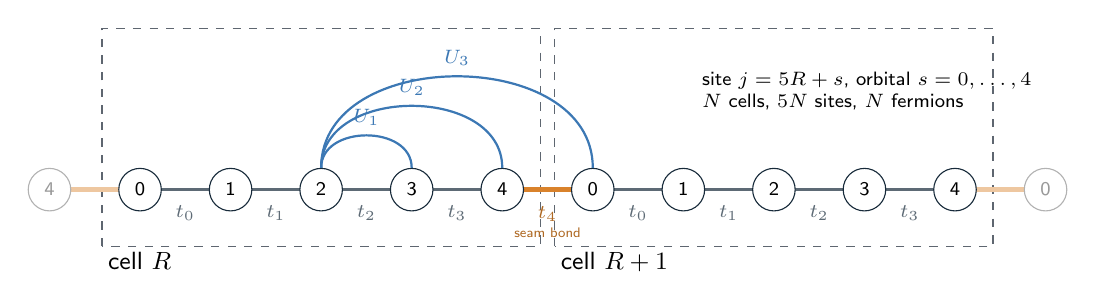
\begin{tikzpicture}[x=11.5mm,y=10mm]
\draw[dashed,rulegray] (-0.42,-0.72) rectangle (4.42,2.05);
\draw[dashed,rulegray] (4.58,-0.72) rectangle (9.42,2.05);
\node[font=\small,anchor=north west,inner sep=2pt] at (-0.42,-0.72) {cell $R$};
\node[font=\small,anchor=north west,inner sep=2pt] at (4.58,-0.72) {cell $R+1$};
\draw[line width=1.6pt,colA!45] (-1,0)--(0,0);
\draw[line width=1.6pt,colA!45] (9,0)--(10,0);
\foreach \x in {0,...,8}{%
  \pgfmathtruncatemacro{\s}{mod(\x,5)}%
  \ifnum\s=4
    \draw[line width=1.6pt,colA] (\x,0)--(\x+1,0) node[midway,below=2pt,font=\scriptsize,text=colA!80!black]{$t_4$};
  \else
    \draw[line width=1pt,ink!70] (\x,0)--(\x+1,0) node[midway,below=2pt,font=\scriptsize]{$t_{\s}$};
  \fi}
\node[font=\tiny,text=colA!80!black] at (4.5,-0.55) {seam bond};
\node[site,faint] at (-1,0) {4};
\node[site,faint] at (10,0) {0};
\foreach \x in {0,...,9}{\pgfmathtruncatemacro{\s}{mod(\x,5)}\node[site] (n\x) at (\x,0) {\s};}
\draw[colB,line width=0.8pt] (n2.north) .. controls +(0,0.55) and +(0,0.55) .. node[pos=0.5,above,font=\scriptsize]{$U_1$} (n3.north);
\draw[colB,line width=0.8pt] (n2.north) .. controls +(0,1.05) and +(0,1.05) .. node[pos=0.5,above,font=\scriptsize]{$U_2$} (n4.north);
\draw[colB,line width=0.8pt] (n2.north) .. controls +(0,1.55) and +(0,1.55) .. node[pos=0.5,above,font=\scriptsize]{$U_3$} (n5.north);
\node[font=\scriptsize,align=left,anchor=west] at (6.1,1.25) {site $j=5R+s$, orbital $s=0,\dots,4$\\ $N$ cells, $5N$ sites, $N$ fermions};
\end{tikzpicture}

\smallskip
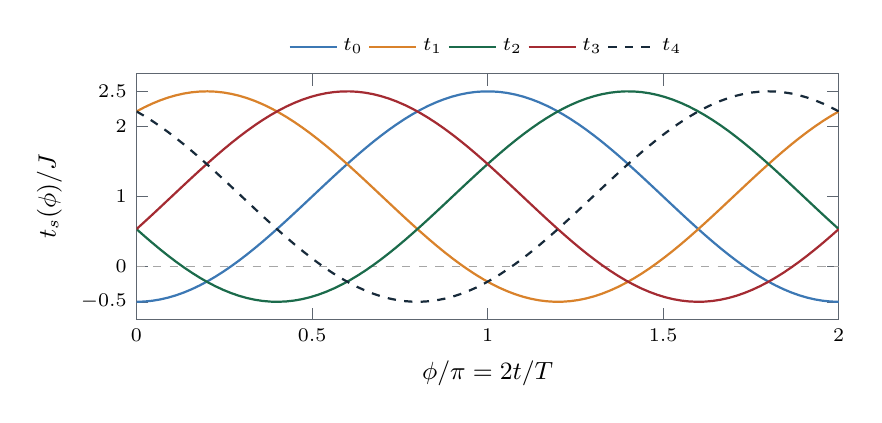
\begin{tikzpicture}
\begin{axis}[mbaxis,width=10.5cm,height=4.7cm,xmin=0,xmax=2,ymin=-0.75,ymax=2.75,
  xlabel={$\phi/\pi=2t/T$},ylabel={$t_s(\phi)/J$},xtick={0,0.5,1,1.5,2},ytick={-0.5,0,1,2,2.5},
  legend columns=5,legend style={at={(0.5,1.03)},anchor=south}]
\addplot[dashed,black!35,domain=0:2,forget plot] {0};
\addplot[colB,thick,domain=0:2,samples=90] {1-1.5*cos(180*x)};
\addplot[colA,thick,domain=0:2,samples=90] {1-1.5*cos(180*x+144)};
\addplot[sourcegreen,thick,domain=0:2,samples=90] {1-1.5*cos(180*x+288)};
\addplot[openred,thick,domain=0:2,samples=90] {1-1.5*cos(180*x+432)};
\addplot[ink,thick,dashed,domain=0:2,samples=90] {1-1.5*cos(180*x+576)};
\legend{$t_0$,$t_1$,$t_2$,$t_3$,$t_4$}
\end{axis}
\end{tikzpicture}
\figtext{\textbf{Top.} Site $j=5R+s$ is orbital $s$ of cell $R$. The bond from orbital $s$ to $s+1$ has hopping $t_s(\phi)$. The orange bond $t_4$ joins orbital 4 of cell $R$ to orbital 0 of cell $R+1$; in M.1 this ``seam'' bond is the one that picks up the factor $e^{\mp ik}$. Blue arcs: the repulsion $U_r$ between two particles $r=1,2,3$ sites apart.
\textbf{Bottom.} The drive at $K/J=-3/2$: the five hoppings as the phase $\phi=2\pi t/T$ advances. After one period every hopping is back to its starting value. The whole problem asks whether particles have nevertheless moved, and for how long that transport survives.}
\end{figpanel}

\smallheading{3. Bands}
Without interactions, translation by one cell is a symmetry. The one-particle problem then reduces to a $5\times5$ matrix $h(k,\phi)$ for each quasi-momentum $k$ (you derive it in M.1). Its five eigenvalues, as functions of $k$, are the five \emph{bands} (Picture~\ref{fig:bands}). At $K/J=-3/2$ the two lowest bands lie close to each other and far below the other three.

\smallheading{4. Localized orbitals and their centres}
From all the Bloch states of one band, or of a group of bands, one can build orbitals that are localized in space, one per cell for each band. They are called \emph{Wannier orbitals}. The expectation value $\langle w|x|w\rangle$ of the position in such an orbital is its \emph{centre}. If every orbital of a set is occupied and every centre moves by $\Delta x$, the transported charge, counted in particles per cell, is $\Delta x/a$, where $a$ is the cell length. Picture~\ref{fig:conveyor}(a): orbitals built from band~1 alone move by $+2$ cells per period. This is an ordinary, integer Thouless pump.

\smallheading{5. Two bands together: flavors and a two-cycle conveyor}
Mixing bands 1 and 2 gives two localized orbitals per cell, called \emph{flavor} $A$ and \emph{flavor} $B$. They can be more compact than orbitals of band 1 alone. Picture~\ref{fig:conveyor}(b) shows the essential geometry: during one period an $A$ orbital slides to the place where a $B$ orbital was. Only after two periods is it back on an $A$ position, one cell to the left. Suppose the particles occupy one flavor only and keep following it. Then every particle moves one cell to the left in two periods: the average transport is $-1/2$ particle per period. This is a \emph{fractional} pump at integer filling.

\smallheading{6. Why interactions matter}
Without interactions the $N$ particles fill band 1, and the pump carries $+2$ particles per period. A strong finite-range repulsion prefers compact, well-separated charges. Occupying one flavor in every cell (all $A$, or all $B$) is then favorable. These two polarized states exchange their roles every period. Exact numerical solutions of small systems [1] show transport of $-1/2$ per period over a range of interaction strengths and drive frequencies. The drive must be slow enough not to excite other states, but fast enough to follow one flavor rather than to tunnel between the all-$A$ and all-$B$ states.

\smallheading{7. The open question}
In a long chain, a region of the other flavor (a \emph{domain}) can appear during the drive. Domains destroy the fractional transport. Reference~[1] expects the fractional pump of a large system to survive only up to some finite time, and leaves that time open. This problem builds and tests the tools one would need to predict that time:
\begin{itemize}[leftmargin=6mm,itemsep=1pt,topsep=2pt]
\item \textbf{Geometry (Parts M, B).} Describe the moving plane of bands 1 and 2 without choosing a basis inside it (a projector $p_{12}$), and how it moves (a generator $g_t$).
\item \textbf{Frames (Part C).} Describe the many-body state in a frame that follows this geometry ($W$) and is dressed by correlations ($e^S$). Keep part of the new generator ($\mathcal K_{\rm ret}$) and bound the rest ($\mathcal R$).
\item \textbf{Current (Part D).} The transported charge is the time integral of the physical current. After a change of frame, the current operator changes too.
\item \textbf{Local errors (Part E).} In a long chain, compare states only in a region $X$ near the place where the current is measured.
\item \textbf{Time (Part F).} Turn error bounds into a statement of the form ``the transported charge stays within the tolerance until time $t$''.
\end{itemize}
Picture~\ref{fig:map} on the reading-map page shows how these steps connect.

\begin{figpanel}{Wannier centres: an integer pump and a two-cycle conveyor}\label{fig:conveyor}
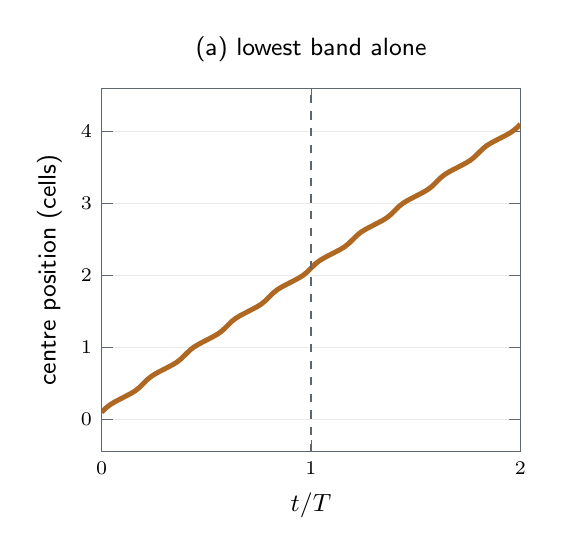
\begin{tikzpicture}
\begin{axis}[mbaxis,width=6.9cm,height=6.2cm,xmin=0,xmax=2,ymin=-0.45,ymax=4.6,
  xlabel={$t/T$},ylabel={centre position (cells)},xtick={0,1,2},ytick={0,1,2,3,4},
  ymajorgrids,grid style={black!8},title={(a) lowest band alone}]
\FigDataBandOne
\draw[dashed,rulegray] (axis cs:1,-0.45)--(axis cs:1,4.6);
\end{axis}
\end{tikzpicture}\hfill
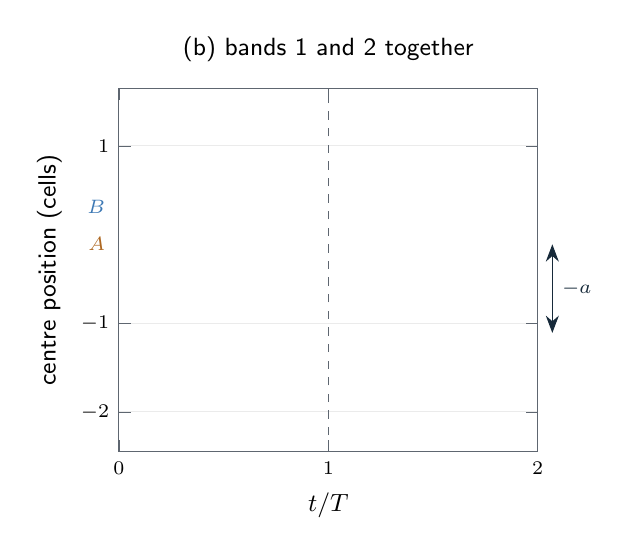
\begin{tikzpicture}
\begin{axis}[mbaxis,width=6.9cm,height=6.2cm,xmin=0,xmax=2,ymin=-2.45,ymax=1.65,clip=false,
  xlabel={$t/T$},ylabel={centre position (cells)},xtick={0,1,2},ytick={-2,-1,1},
  ymajorgrids,grid style={black!8},title={(b) bands 1 and 2 together}]
\FigDataComposite
\draw[dashed,rulegray] (axis cs:1,-2.45)--(axis cs:1,1.65);
\node[font=\scriptsize\bfseries,text=colA!80!black,anchor=east] at (axis cs:-0.02,-0.11) {$A$};
\node[font=\scriptsize\bfseries,text=colB,anchor=east] at (axis cs:-0.02,0.31) {$B$};
\draw[<->,ink] (axis cs:2.07,-0.11)--(axis cs:2.07,-1.11) node[midway,right,font=\scriptsize]{$-a$};
\end{axis}
\end{tikzpicture}
\figtext{Computed for this booklet from $h(k,\phi)$ at $K/J=-3/2$: centres of the localized (Wannier) orbitals, obtained from the projected position operator on a 24-cell ring. This is single-particle geometry only; no interacting dynamics is computed.
(a) One orbital per cell built from band 1 alone: it moves by an integer number of cells per period (an ordinary Thouless pump).
(b) Two orbitals per cell built from bands 1 and 2 together: flavor $A$ (orange) and flavor $B$ (blue). Follow the thick curve. It does not return to an $A$ position after one period; it returns only after two periods, one cell to the left ($-a$).
\textbf{A.1 asks:} if every particle rides a curve like the thick one, how much charge has passed after $2T$, and per period on average? Whether interacting particles really stay on one such curve is the open question of the whole problem.}
\end{figpanel}

\begin{figpanel}{M.1 --- the five single-particle bands at $K/J=-3/2$}\label{fig:bands}
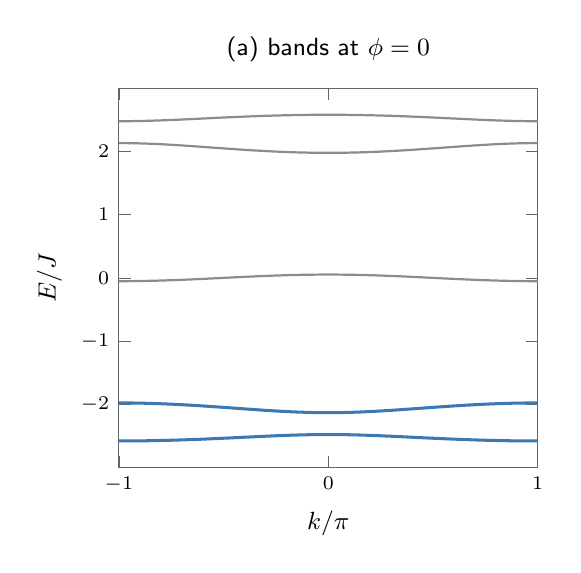
\begin{tikzpicture}
\begin{axis}[mbaxis,width=6.9cm,height=6.4cm,xmin=-1,xmax=1,ymin=-3,ymax=3,
  xlabel={$k/\pi$},ylabel={$E/J$},xtick={-1,0,1},ytick={-2,-1,0,1,2},title={(a) bands at $\phi=0$}]
\FigDataBandsK
\end{axis}
\end{tikzpicture}\hfill
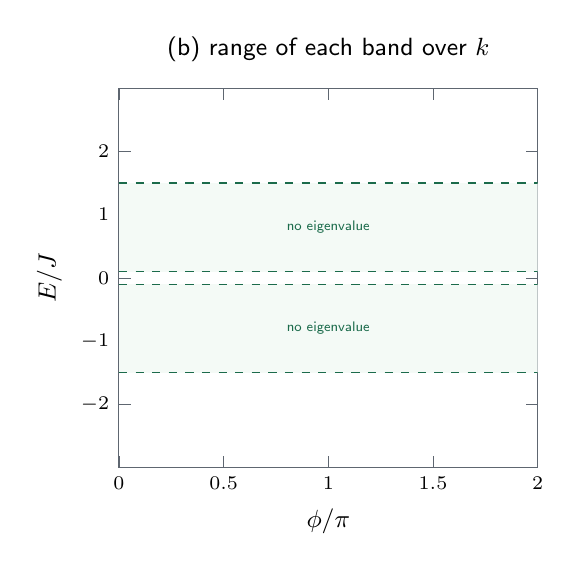
\begin{tikzpicture}
\begin{axis}[mbaxis,width=6.9cm,height=6.4cm,xmin=0,xmax=2,ymin=-3,ymax=3,
  xlabel={$\phi/\pi$},ylabel={$E/J$},xtick={0,0.5,1,1.5,2},ytick={-2,-1,0,1,2},title={(b) range of each band over $k$}]
\fill[sourcewash] (axis cs:0,-1.5) rectangle (axis cs:2,-0.1);
\fill[sourcewash] (axis cs:0,0.1) rectangle (axis cs:2,1.5);
\FigDataBandsPhi
\draw[dashed,sourcegreen] (axis cs:0,-1.5)--(axis cs:2,-1.5);
\draw[dashed,sourcegreen] (axis cs:0,-0.1)--(axis cs:2,-0.1);
\draw[dashed,sourcegreen] (axis cs:0,0.1)--(axis cs:2,0.1);
\draw[dashed,sourcegreen] (axis cs:0,1.5)--(axis cs:2,1.5);
\node[font=\tiny,text=sourcegreen] at (axis cs:1,-0.8) {no eigenvalue};
\node[font=\tiny,text=sourcegreen] at (axis cs:1,0.8) {no eigenvalue};
\end{axis}
\end{tikzpicture}
\figtext{Computed for this booklet from $h(k,\phi)$. Blue: the two lowest bands, treated together as one group; $p_{12}(k,\phi)$ projects onto this blue pair. Grey: bands 3--5.
\textbf{M.1 asks} you to derive the $5\times5$ matrix whose eigenvalues are these curves, and to build $p_{12}$ from the two blue eigenvectors.
No eigenvalue enters the two green windows: the blue group stays well separated from band 3 (numerically by about $1.9J$).}
\end{figpanel}

\nextpage
\pagetitle{Toolkit. Facts you may use without proof}
\label{toolkit}
{\small
\begin{enumerate}[label=\textbf{T\arabic*.},leftmargin=9mm,itemsep=4pt,topsep=2pt]
\item \textbf{Projectors.} An orthogonal projector obeys $p^2=p=p^\dagger$. Its rank is $\Tr p$.
\item \textbf{Change of frame.} If $i\partial_t\ket\psi=H\ket\psi$ and $\ket\xi=U^\dagger\ket\psi$ with a differentiable unitary $U(t)$, then $i\partial_t\ket\xi=(U^\dagger HU-iU^\dagger\dot U)\ket\xi$.
\item \textbf{Time-dependent operators.} If $i\partial_t\ket\xi=\mathcal K\ket\xi$ and $O(t)$ is an operator, then $\frac{\dd}{\dd t}\bra\xi O\ket\xi=\bra\xi\big(\partial_tO+i[\mathcal K,O]\big)\ket\xi$.
\item \textbf{Pauli matrices.} $\sigma_a\sigma_b=\delta_{ab}\id+i\epsilon_{abc}\sigma_c$; for example $[\sigma_z,\sigma_x]=2i\sigma_y$. For a unit vector $\bm n$: $e^{ix\bm n\cdot\bm\sigma}=\id\cos x+i(\bm n\cdot\bm\sigma)\sin x$. Operators on different spins commute.
\item \textbf{Norms.} $\norm A$ is the operator norm (largest singular value); $\norm A_1$ is the trace norm (sum of singular values). Then $\norm{AB}\le\norm A\norm B$, $\norm{[A,B]}\le2\norm A\norm B$, and $|\Tr(AB)|\le\norm A_1\norm B$. For density matrices $\norm{\rho-\sigma}_1\le2$.
\item \textbf{Reduced states.} Split a system into a region $X$ and the rest $\bar X$. The reduced state is $\rho_X=\Tr_{\bar X}\rho$ (trace over $\bar X$ only). If $O_X$ acts only on $X$, then $\Tr(\rho O_X)=\Tr_X(\rho_XO_X)$ and $\Tr_{\bar X}(O_X\rho)=O_X\rho_X$.
\item \textbf{Fermion modes.} $\{c_x,c_y^\dagger\}=\delta_{xy}$. For a one-particle vector $f$, $a(f)=\sum_xf_x^*c_x$ removes a particle from orbital $f$, and $\norm{a(f)}=\norm f$. A one-particle matrix $A$ becomes the many-body operator $\widehat A=\sum_{xy}A_{xy}c_x^\dagger c_y$. A one-particle unitary $U$ becomes a many-body unitary $\Gamma(U)$ that maps each $c_x^\dagger$ to $\sum_yU_{yx}c_y^\dagger$; it conserves particle number.
\item \textbf{Counting.} $N$ fermions in $M$ distinct modes can be placed in $\binom MN$ ways.
\item \textbf{Resolvent.} For a Hermitian matrix $h$, $\norm{(\zeta-h)^{-1}}=1/\operatorname{dist}(\zeta,\text{spectrum of }h)$. If a closed contour $\mathscr C$ encloses some eigenvalues and no others, $\frac1{2\pi i}\oint_{\mathscr C}(\zeta-h)^{-1}\dd\zeta$ is the projector onto their eigenvectors.
\item \textbf{Fourier coefficients.} For a $2\pi$-periodic matrix function $f(k)$, $f_R=\int_{-\pi}^{\pi}\frac{\dd k}{2\pi}e^{ikR}f(k)$ and $\norm{f_R}\le\int\frac{\dd k}{2\pi}\norm{f(k)}$. If $f$ extends analytically to the strip $|\operatorname{Im}k|\le\kappa$, the integration line may be moved to $\operatorname{Im}k=\pm\kappa$.
\item \textbf{Wannier centres in one dimension.} On a ring of length $L$, let $P$ project onto the occupied one-particle states of a group of bands. For a long ring, the eigenvalues of $Pe^{2\pi ix/L}P$ on the range of $P$ are close to $e^{2\pi ix_\alpha/L}$, where $x_\alpha$ are the centres of the maximally localized orbitals of that group. In momentum space this operator is the \emph{Wilson loop}: the ordered product of the overlaps of the band eigenvectors around the Brillouin zone, at fixed drive phase $\phi$.
\end{enumerate}}

\nextpage
\pagetitle{Glossary}
\label{glossary}
{\small\begin{tabularx}{\textwidth}{@{}>{\bfseries}p{34mm}Y@{}}\toprule
Band; Bloch matrix&The eigenvalues $E_n(k,\phi)$ of the one-particle matrix $h(k,\phi)$; $h$ itself (M.1).\\
Composite bands&Bands 1 and 2 treated as one group, without separating them.\\
Projector $p_{12}$&The projector onto the plane spanned by the band-1 and band-2 eigenvectors at given $(k,\phi)$. $\operatorname{Gr}(2,5)$ is the set of all planes (2-dimensional subspaces) in $\mathbb C^5$.\\
Wannier orbital, centre&A localized orbital built from Bloch states; its mean position.\\
Flavor $A$, $B$&The two localized orbitals per cell built from bands 1 and 2.\\
Seam&(i) The bond $t_4$ between neighbouring cells. (ii) In time: the matching at $t=T$, where the labels $A$ and $B$ exchange.\\
Reference state&A simple state that the true state is compared with, e.g.\ all particles in flavor $A$.\\
Moving frame $W(t)$&A unitary that follows the geometry; the state is described relative to it (T2).\\
Dressing $e^S$&A further unitary, with $S$ anti-Hermitian, that builds correlations into the reference.\\
$\mathcal K_{\rm ret}$, $\mathcal R$&The part of the transformed generator that is kept, and the part that is omitted.\\
Slater determinant; single/double excitation&A state of independent fermions in chosen orbitals; the same state with one or two orbitals replaced by others.\\
External weight&The probability that a state lies outside a chosen reference space.\\
Reduced state; partial trace&See T6.\\
Trace distance&$\norm{\rho-\sigma}_1$: how well two states can be told apart by any measurement (at most 2).\\
Fidelity&$\mathcal F(\rho,\ket a)=\bra a\rho\ket a$ (E.1).\\
Window charge $\Qbar(t)$&Charge per period, averaged over the two periods that end at $t$ (Part F).\\
MB1&The research project behind this problem: the original MFP pump at $K/J=-3/2$.\\
\bottomrule
\end{tabularx}}

\nextpage
\pagetitle{Reading map. What is the object at each step?}
\label{route-map}
\textbf{Research target:} predict when the original interacting pump leaves a chosen charge tolerance, and identify the process that controls that change. A guaranteed interval is useful, but is not automatically the actual first-failure time.

\begin{figpanel}{The chain of objects used in this problem}\label{fig:map}
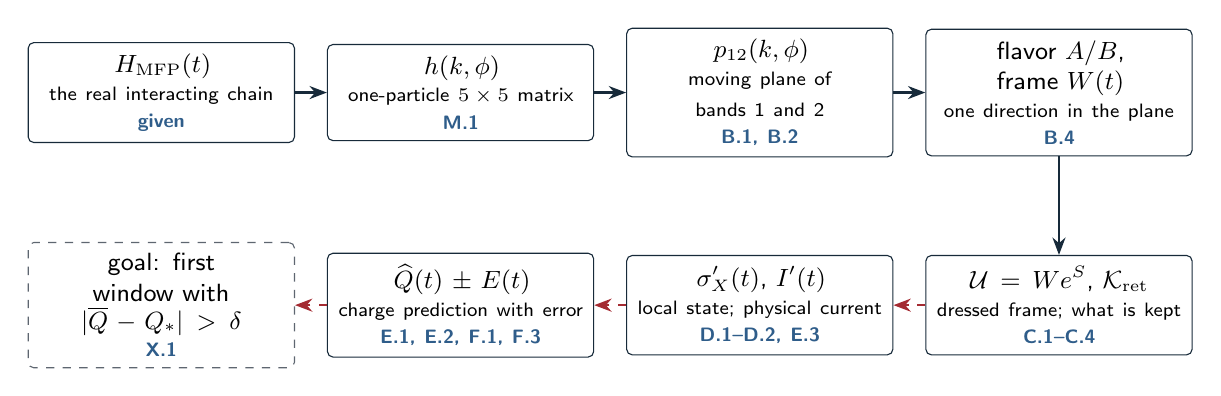
\begin{tikzpicture}[x=1mm,y=1mm]
\node[obj] (n1) at (0,0) {$H_{\rm MFP}(t)$\\[-1pt]{\scriptsize the real interacting chain}\\[-1pt]\ftag{given}};
\node[obj] (n2) at (38,0) {$h(k,\phi)$\\[-1pt]{\scriptsize one-particle $5\times5$ matrix}\\[-1pt]\ftag{M.1}};
\node[obj] (n3) at (76,0) {$p_{12}(k,\phi)$\\[-1pt]{\scriptsize moving plane of bands 1 and 2}\\[-1pt]\ftag{B.1, B.2}};
\node[obj] (n4) at (114,0) {flavor $A/B$, frame $W(t)$\\[-1pt]{\scriptsize one direction in the plane}\\[-1pt]\ftag{B.4}};
\node[obj] (n5) at (114,-27) {$\mathcal U=We^{S}$, $\mathcal K_{\rm ret}$\\[-1pt]{\scriptsize dressed frame; what is kept}\\[-1pt]\ftag{C.1--C.4}};
\node[obj] (n6) at (76,-27) {$\sigma'_X(t)$, $I'(t)$\\[-1pt]{\scriptsize local state; physical current}\\[-1pt]\ftag{D.1--D.2, E.3}};
\node[obj] (n7) at (38,-27) {$\widehat Q(t)\pm E(t)$\\[-1pt]{\scriptsize charge prediction with error}\\[-1pt]\ftag{E.1, E.2, F.1, F.3}};
\node[obj,dashed,draw=rulegray] (n8) at (0,-27) {goal: first window with\\[-1pt]$|\Qbar-Q_*|>\delta$\\[-1pt]\ftag{X.1}};
\draw[okarrow] (n1)--(n2);
\draw[okarrow] (n2)--(n3);
\draw[okarrow] (n3)--(n4);
\draw[okarrow] (n4)--(n5);
\draw[openarrow] (n5)--(n6);
\draw[openarrow] (n6)--(n7);
\draw[openarrow] (n7)--(n8);
\end{tikzpicture}
\figtext{Read the boxes in the order of the arrows. Each box is a mathematical object; the blue label says which questions work with it. Black arrows are steps that this booklet derives. Red dashed arrows are links that are \emph{not yet established} for the original pump; several questions ask why. The interactions of $H_{\rm MFP}$ are not lost after the first arrow: they come back in Part C.}
\end{figpanel}

\begin{center}\small
\begin{tabularx}{\textwidth}{@{}>{\raggedright\arraybackslash}p{25mm}Y>{\raggedright\arraybackslash}p{34mm}@{}}\toprule
Step&Why the next object is needed&Questions\\ \midrule
Target&Ideal winding must be distinguished from actual following.&A.1--A.2\\
Model object&Five Bloch components are not the full many-body state. Select the composite bands for a physical reason.&M.1\\
Geometry&Compare a moving subspace without choosing arbitrary basis vectors. Then resolve its internal flavor.&B.1, B.2, B.4\\
Dynamics&A change of frame does not by itself remove interactions. Decide what to keep and what to bound.&C.1--C.4\\
Current&Use the transformed physical current, not a population count.&D.1--D.2\\
Local state&The kept Hamiltonian must actually determine local occupations and coherences.&E.1--E.3\\
Time&Convert local-state and current errors into a charge interval.&F.1, F.3, X.1\\ \bottomrule
\end{tabularx}
\end{center}

\begin{redbox}{OPEN --- the central dynamical link}
The reference evolution and its local error are not yet controlled over the full drive. In particular, $\mathcal K_{\rm ret}\to\sigma'_X\to\widehat Q$ is not supplied by the composite-band geometry.
\end{redbox}
\origin{Recommended route: A $\to$ M $\to$ B $\to$ C $\to$ D $\to$ E $\to$ F $\to$ X.}

\nextpage
\parttitle{A}{Fractional transport and domain energy}{1.5}

\begin{greenbox}{MFP [1] --- a candidate two-cycle branch}
The two Wannier flavors may exchange after one period. In the source argument, a continuously followed flavor returns after two periods with a one-cell displacement (Background~\S5, Picture~\ref{fig:conveyor}). The argument assumes that the occupations continue to follow that branch.
\end{greenbox}

\begin{redbox}{ADDED IDEAL-FOLLOWING CONDITION}
For A.1, stipulate that the actual occupied orbitals follow the branch exactly. This is not a large-system finite-speed stability result.

An $N$-cell ring has cell length $a$ and contains $N$ particles. After $2T$, each occupied orbital has an unwrapped center displacement $\Delta x_j=-a$. Define the spatially averaged transported particle number by
\[
Q(0,2T)=\frac{1}{Na}\sum_{j=1}^{N}\Delta x_j.
\]
The single-period values $Q(0,T)$ and $Q(T,2T)$ are defined in the same way from the displacements during each period.
\end{redbox}
\question{A.1}{0.6}{Find $Q(0,2T)$ and the transport per drive period, averaged over these two periods. Must the two single-period values each equal $-1/2$? Explain.}

\par\Needspace{34\baselineskip}
\begin{redbox}{ADDED MODEL --- a spin-chain analogy}
For A.2 only, replace the pump by the model below. Its parameters are not identified with $K$ or $U_r$. This model explains an energy competition; it is not a controlled reduction of MFP.

\[
H_{\rm d}=-J_z\sum_j\sigma_j^z\sigma_{j+1}^z
-h\sum_j\sigma_j^z-g\sum_j\sigma_j^x,
\qquad J_z,h>0.
\]
Let $A$ mean $\sigma^z=-1$ and $B$ mean $\sigma^z=+1$. Set $g=0$. Start with all spins in $A$. Flip a consecutive segment of $\ell$ spins to $B$, with $1\leq\ell<N$. There are two interfaces between the segment and its surroundings.

\end{redbox}
\begin{figpanel}{A.2 --- a domain in the teaching spin chain}\label{fig:domain}
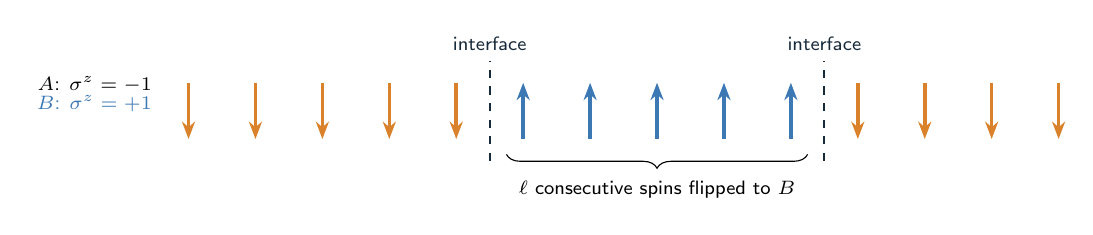
\begin{tikzpicture}[x=8.5mm,y=8.5mm]
\foreach \x in {0,...,13}{%
  \ifnum\x>4 \ifnum\x<10
    \draw[->,line width=1.3pt,colB] (\x,-0.42)--(\x,0.42);
  \else
    \draw[->,line width=1.3pt,colA] (\x,0.42)--(\x,-0.42);
  \fi\else
    \draw[->,line width=1.3pt,colA] (\x,0.42)--(\x,-0.42);
  \fi}
\draw[ink,dashed,line width=0.8pt] (4.5,-0.75)--(4.5,0.75) node[above,font=\scriptsize]{interface};
\draw[ink,dashed,line width=0.8pt] (9.5,-0.75)--(9.5,0.75) node[above,font=\scriptsize]{interface};
\draw[decorate,decoration={brace,amplitude=5pt,mirror}] (4.75,-0.65)--(9.25,-0.65) node[midway,below=6pt,font=\scriptsize]{$\ell$ consecutive spins flipped to $B$};
\node[font=\scriptsize,anchor=east,align=right] at (-0.4,0.25) {$A$: $\sigma^z=-1$\\[-1pt]{\color{colB}$B$: $\sigma^z=+1$}};
\end{tikzpicture}
\figtext{Orange arrows: $A$ ($\sigma^z=-1$). Blue arrows: $B$ ($\sigma^z=+1$). \textbf{A.2 asks:} (i) the energy bookkeeping --- how much each of the two interfaces costs through the $J_z$ term and how much each flipped spin changes through the $h$ term; (ii) the shortest segment that lowers the energy; (iii) whether lower energy alone forces an isolated chain that starts all-$A$ to produce such a segment when $g=0$.}
\end{figpanel}

\question{A.2}{0.9}{Find the energy change $\Delta E(\ell)$. Find the smallest integer $\ell$ for which it is strictly negative, provided that segment fits in the chain. Does an isolated system initially in the all-$A$ state then have to form this lower-energy domain when $g=0$?}


\nextpage
\parttitle{M}{From the lattice to the geometric object}{1.0}
\begin{greenbox}{MFP [1], Eq.~(1)--(2) --- source model and motivation}
In the source mechanism, mixing the lowest two bands permits more localized Wannier orbitals, and finite-range repulsion can favor occupation of one flavor (Background~\S5--6).
\end{greenbox}

\smallheading{M.1 input: fix the representation before choosing a projector}
Write the physical site index as $j=5R+s$, with cell $R$ and orbital $s=0,\ldots,4$. Define
\[
t_s(\phi)=J+K\cos(\phi+4\pi s/5),\qquad
c_{R,s}=\frac1{\sqrt N}\sum_k e^{ikR}c_{k,s},
\]
where $k=2\pi m/N$ is a dimensionless cell momentum. The single-particle part is
\[
H_0=-\sum_R\left[\sum_{s=0}^{3}t_s c_{R,s+1}^\dagger c_{R,s}
+t_4c_{R+1,0}^\dagger c_{R,4}+\hc\right].
\]
The full model remains $H_{\rm MFP}=H_0+H_{\rm int}$.

\begin{figpanel}{M.1(c) --- three different ways to place $N=4$ particles in $N=4$ cells}\label{fig:counting}
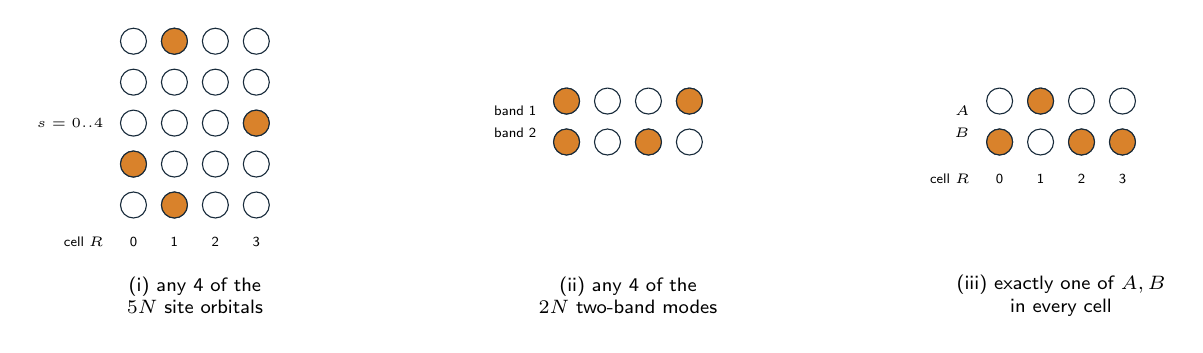
\begin{tikzpicture}[x=5.2mm,y=5.2mm,dot/.style={circle,draw=ink,inner sep=0pt,minimum size=3.3mm},full/.style={dot,fill=colA}]
\begin{scope}
\foreach \c in {0,...,3}\foreach \r in {0,...,4}{\node[dot] at (\c,\r) {};}
\foreach \c/\r in {0/1,1/0,1/4,3/2}{\node[full] at (\c,\r) {};}
\foreach \c in {0,...,3}{\node[font=\tiny] at (\c,-0.9) {\c};}\node[font=\tiny,anchor=east] at (-0.5,-0.9) {cell $R$};
\node[font=\tiny,anchor=east] at (-0.5,2) {$s=0..4$};
\node[font=\scriptsize,align=center] at (1.5,-2.2) {(i) any 4 of the\\ $5N$ site orbitals};
\end{scope}
\begin{scope}[xshift=55mm,yshift=8mm]
\foreach \c in {0,...,3}\foreach \r in {0,1}{\node[dot] at (\c,\r) {};}
\foreach \c/\r in {0/0,0/1,2/0,3/1}{\node[full] at (\c,\r) {};}
\node[font=\tiny,anchor=east,align=right] at (-0.5,0.5) {band 1\\[2pt] band 2};
\node[font=\scriptsize,align=center] at (1.5,-3.75) {(ii) any 4 of the\\ $2N$ two-band modes};
\end{scope}
\begin{scope}[xshift=110mm,yshift=8mm]
\foreach \c in {0,...,3}\foreach \r in {0,1}{\node[dot] at (\c,\r) {};}
\foreach \c/\r in {0/0,1/1,2/0,3/0}{\node[full] at (\c,\r) {};}
\foreach \c in {0,...,3}{\node[font=\tiny] at (\c,-0.9) {\c};}\node[font=\tiny,anchor=east] at (-0.5,-0.9) {cell $R$};
\node[font=\tiny,anchor=east,align=right] at (-0.5,0.5) {$A$\\[2pt] $B$};
\node[font=\scriptsize,align=center] at (1.5,-3.75) {(iii) exactly one of $A,B$\\ in every cell};
\end{scope}
\end{tikzpicture}
\figtext{Filled circles: occupied single-particle states (one example pattern each). \textbf{M.1(c) asks} you to count all allowed patterns in each picture, and to say which physical restriction each picture imposes. Only after that can you judge whether Fourier transformation has reduced the many-body problem.}
\end{figpanel}

\bridge{M.1}{1.0}{\textbf{(a)} Derive the $5\times5$ matrix $h(k,\phi)$ in the ordered basis $(0,1,2,3,4)$. Check both complex seam entries and Hermiticity for real $k$.\par
\textbf{(b)} Let $Y=(\ket{u_1},\ket{u_2})$ contain two orthonormal lowest-band eigenvectors. Construct $p_{12}=YY^\dagger$. Find its rank and ambient dimension. Why is this object physically motivated in MFP?\par
\textbf{(c)} Compare $\binom{5N}{N}$, $\binom{2N}{N}$, and $2^N$. State the different restrictions behind them. Evaluate all three at $N=4$. Has Fourier transformation solved the many-body problem?}

\hint{Insert the Fourier expansion into each term of $H_0$ and use $\frac1N\sum_Re^{i(k'-k)R}=\delta_{kk'}$. Write $H_0=\sum_k\bm c_k^\dagger h(k,\phi)\bm c_k$ with $\bm c_k=(c_{k,0},\dots,c_{k,4})^{T}$.}

\smallheading{Useful counting rule}
Choosing $N$ occupied modes among $M$ distinct fermionic modes gives $\binom MN$ occupation states. Exactly one occupied flavor per cell is an additional restriction, not the same as average filling one.


\begin{redbox}{OPEN --- a reference choice is not a dynamical truncation}
The two-band $N$-particle sector is not a two-state system. Restricting the full interacting model to this sector requires control of the terms that leave it.
\end{redbox}
\handoff{The physical output is a defined composite-band projector. Part B describes its motion. B.4 then asks how to identify a flavor inside it.}

\nextpage
\parttitle{B}{Geometry and actual motion}{2.2}
\begin{greenbox}{H2 [2] --- projector kinematics}
A projector represents a subspace without choosing a basis inside it. Its derivative describes the change of that subspace. In B.1, derive the corresponding horizontal generator. This is a kinematic statement, not a lifetime prediction.

Let $p(t)$ be a smooth orthogonal projector, so $p^2=p=p^\dagger$.
\end{greenbox}
\begin{figpanel}{B.1 and B.2 --- a moving projector and one spin in a turning field}\label{fig:bloch}
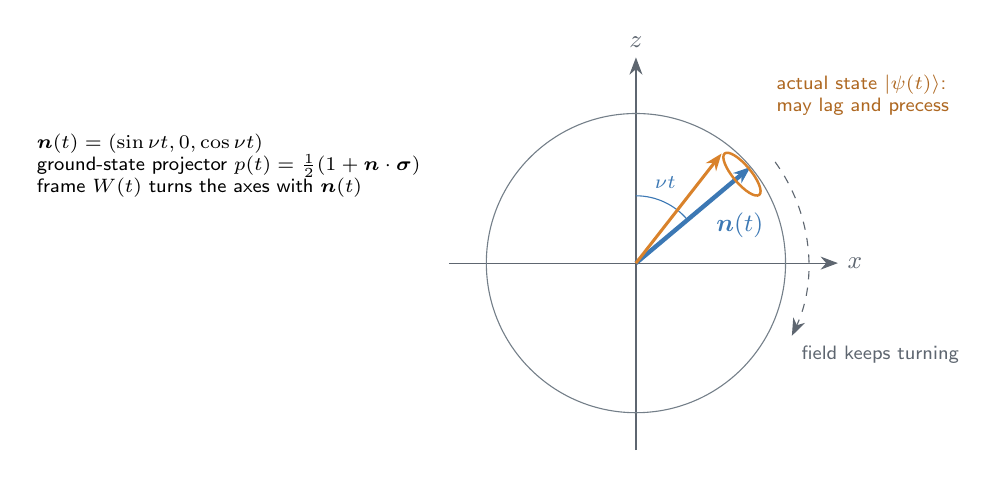
\begin{tikzpicture}[scale=0.95]
\draw[->,rulegray] (-2.5,0)--(2.7,0) node[right,font=\small]{$x$};
\draw[->,rulegray] (0,-2.5)--(0,2.75) node[above,font=\small]{$z$};
\draw[ink!60] (0,0) circle (2);
\draw[->,dashed,rulegray] (36:2.3) arc (36:-25:2.3) node[below right,font=\scriptsize]{field keeps turning};
\draw[colB] (90:0.9) arc (90:40:0.9);
\node[font=\scriptsize,text=colB] at (70:1.15) {$\nu t$};
\draw[->,line width=1.6pt,colB] (0,0)--(40:2) node[pos=0.62,below right=-1pt,font=\small]{$\bm n(t)$};
\draw[colA,line width=0.9pt,rotate around={-50:(40:1.85)}] (40:1.85) ellipse (0.36 and 0.12);
\draw[->,line width=1.1pt,colA] (0,0)--(52:1.86);
\node[font=\scriptsize,text=colA!80!black,align=left,anchor=west] at (1.75,2.25) {actual state $\ket{\psi(t)}$:\\ may lag and precess};
\node[font=\scriptsize,align=left,anchor=east] at (-2.75,1.3) {$\bm n(t)=(\sin\nu t,0,\cos\nu t)$\\ ground-state projector $p(t)=\tfrac12(\id+\bm n\cdot\bm\sigma)$\\ frame $W(t)$ turns the axes with $\bm n(t)$};
\end{tikzpicture}
\figtext{The circle is a cut through the Bloch sphere. The field direction $\bm n(t)$ (blue) turns at rate $\nu$; its size $\Delta$ is fixed. The instantaneous ground state points along $\bm n$, which is the projector path $p(t)$. \textbf{B.1 asks} for a generator $g_t$ that is built from the path $p(t)$ alone and moves it correctly. \textbf{B.2 asks} you to go to the frame that turns with $\bm n(t)$, find the Hamiltonian there, and from it the probability that the orange state is found in the excited state. The path depends only on $\nu$; the question is what $\Delta$ does.}
\end{figpanel}

\question{B.1}{0.5}{Show that $p\dot p\,p=0$. Define $g_t=i[\dot p,p]$ and prove $[g_t,p]=i\dot p$. State what this identity determines and what it does not determine about the actual Hamiltonian.}

\begin{redbox}{ADDED MODEL --- an exactly solvable rotating spin}
For B.2, study one spin. This is a test of moving-frame dynamics, not the complete interacting pump.

\[
H(t)=-\frac{\Delta}{2}
\big[\sin(\nu t)\sigma_x+\cos(\nu t)\sigma_z\big],
\qquad \Delta,\nu>0.
\]
Its instantaneous ground-state projector and a rotating frame are
\[
\begin{split}
p(t)&=\tfrac12\big[\id+\sin(\nu t)\sigma_x+\cos(\nu t)\sigma_z\big],\\
W(t)&=e^{-i\nu t\sigma_y/2},\qquad
\ket{\Xi(t)}=W^\dagger(t)\ket{\psi(t)}.
\end{split}
\]
Use $\ket{\psi(0)}=\ket{\uparrow}$, where $\sigma_z\ket{\uparrow}=\ket{\uparrow}$.

\end{redbox}
\question{B.2}{0.9}{Find the time-independent moving-frame Hamiltonian $\mathcal K=W^\dagger HW-iW^\dagger\dot W$. Find the exact probability $P_{\rm ex}(t)$ of occupying the instantaneous excited state. Explain how changing $\Delta$ can change this probability without changing the projector path.}

\smallheading{Useful identity}
For a unit vector $\bm n$ and real $x$,
\[
e^{ix\bm n\cdot\bm\sigma}=\id\cos x+i(\bm n\cdot\bm\sigma)\sin x.
\]
\origin{B.1 uses H2. B.2 is a teaching construction. Its exact solution does not prove a regime of the original pump.}

\par\Needspace{14\baselineskip}\bigskip
\pagetitle{B.4. A plane is not yet a flavor}
\begin{greenbox}{MFP [1], Eq.~(2); H2 [2] --- two linked objects}
The source chooses localized Wannier flavors inside the composite bands. H2 describes the composite projector without an arbitrary internal basis. A physical flavor requires a localization rule and continuous tracking, not just the endpoint statement $p_{12}(T)=p_{12}(0)$.
\end{greenbox}
Let $Y(k,\phi)=(\ket{u_1},\ket{u_2})$ and let $V(k,\phi)$ be a unitary $2\times2$ matrix. If $v_\alpha$ is its column, define
\[
u_\alpha=Yv_\alpha,\qquad
p_\alpha=Yv_\alpha v_\alpha^\dagger Y^\dagger,\qquad\alpha=A,B.
\]
The source's Wannier construction has the form
\[
\ket{w_{R,\alpha}}=\frac1{\sqrt N}\sum_{k,n=1,2}
 e^{-ikR}V_{n\alpha}(k,\phi)\ket{\psi_{kn}(\phi)}.
\]
Here $\ket{\psi_{kn}}$ is a full Bloch state. Its physical center uses the actual site positions $x_{R,s}=Ra+r_s$. The Wilson loop is described in T11.

\bridge{B.4}{0.8}{\textbf{(a)} Show that replacing $Y$ by $Y\Lambda$ for any unitary $\Lambda$ leaves $p_{12}$ unchanged. Show that a fixed physical $p_A$ also stays unchanged if $v_A\to \Lambda^\dagger v_A$. What changes if one selects a different internal direction without this compensation?\par
\textbf{(b)} Explain what must be evaluated to obtain the centers $\langle w_{R,\alpha}|x|w_{R,\alpha}\rangle$ and a continuously labelled A/B path. Distinguish the Wilson loop around $k$ from evolution over physical time.\par
\textbf{(c)} Use the added counterexample below. Does a closed composite projector or a determinant phase determine internal exchange? Does internal exchange alone prove charge transport?}

\begin{redbox}{ADDED COUNTEREXAMPLE --- not computed MFP matrices}
In a physically labelled two-dimensional space, compare $\mathscr T_0=\id_2$ with $\mathscr T_1=i\sigma_x$. Both act inside the same plane. No real-space displacement is specified. These are illustrative internal maps, not the original pump's Wilson or evolution matrices.
\end{redbox}

\begin{figpanel}{B.4 --- a plane is not yet a flavor}\label{fig:plane}
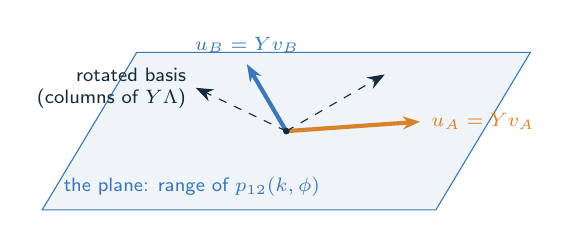
\begin{tikzpicture}[x=10mm,y=10mm]
\fill[colB!8,draw=colB] (0,0)--(5,0)--(6.2,2)--(1.2,2)--cycle;
\node[font=\scriptsize,text=colB,anchor=south west] at (0.15,0.05) {the plane: range of $p_{12}(k,\phi)$};
\coordinate (O) at (3.1,1.0);
\draw[->,line width=1.5pt,colA] (O)--++(1.7,0.12) node[right,font=\scriptsize]{$u_A=Yv_A$};
\draw[->,line width=1.5pt,colB] (O)--++(-0.5,0.85) node[above,font=\scriptsize]{$u_B=Yv_B$};
\draw[->,dashed,ink] (O)--++(1.25,0.72);
\draw[->,dashed,ink] (O)--++(-1.15,0.55) node[left,font=\scriptsize,align=right]{rotated basis\\(columns of $Y\Lambda$)};
\fill[ink] (O) circle (1.2pt);
\end{tikzpicture}\hspace{8mm}
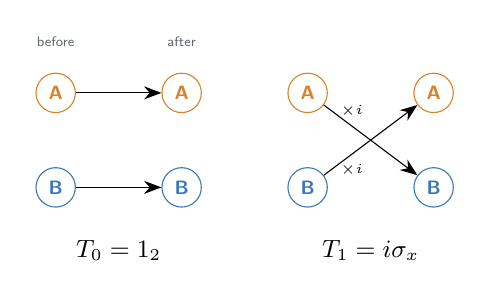
\begin{tikzpicture}[x=10mm,y=10mm,st/.style={circle,draw,inner sep=1pt,minimum size=5mm,font=\scriptsize\bfseries}]
\node[st,draw=colA,text=colA] (a0) at (0,1.2) {A};
\node[st,draw=colB,text=colB] (b0) at (0,0) {B};
\node[st,draw=colA,text=colA] (a1) at (1.6,1.2) {A};
\node[st,draw=colB,text=colB] (b1) at (1.6,0) {B};
\draw[->] (a0)--(a1); \draw[->] (b0)--(b1);
\node[font=\small] at (0.8,-0.8) {$\mathscr T_0=\id_2$};
\node[st,draw=colA,text=colA] (c0) at (3.2,1.2) {A};
\node[st,draw=colB,text=colB] (d0) at (3.2,0) {B};
\node[st,draw=colA,text=colA] (c1) at (4.8,1.2) {A};
\node[st,draw=colB,text=colB] (d1) at (4.8,0) {B};
\draw[->] (c0)--(d1) node[pos=0.3,above,font=\tiny]{$\times i$};
\draw[->] (d0)--(c1) node[pos=0.3,below,font=\tiny]{$\times i$};
\node[font=\small] at (4.0,-0.8) {$\mathscr T_1=i\sigma_x$};
\node[font=\tiny,text=rulegray] at (0,1.85) {before};
\node[font=\tiny,text=rulegray] at (1.6,1.85) {after};
\end{tikzpicture}
\figtext{\textbf{Left.} The two lowest bands span a plane at each $(k,\phi)$. Inside it one can pick two orthonormal directions $u_A,u_B$ (the flavors), or any rotated pair. \textbf{B.4(a) asks} which choices change only the coordinates and which change a physical object. \textbf{B.4(b) asks} what extra information --- a localization rule, the real site positions, continuous tracking in time --- turns the plane into labelled $A/B$ orbitals with centres. \textbf{Right.} Two internal maps of the same plane. \textbf{B.4(c) asks} whether one number such as a determinant phase can tell $\mathscr T_0$ from $\mathscr T_1$, and whether swapping $A$ and $B$ by itself moves charge.}
\end{figpanel}

\nextpage
\parttitle{C}{Correlation and overlapping local corrections}{3.9}
\begin{figpanel}{C.1 and C.2 --- one correlation channel; two overlapping corrections}\label{fig:cone}
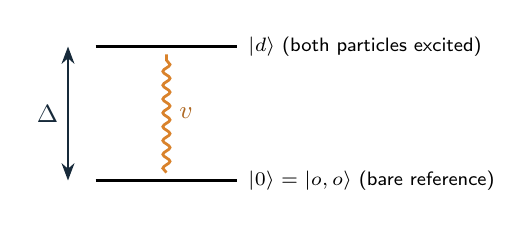
\begin{tikzpicture}[x=10mm,y=10mm]
\draw[line width=1.2pt] (0,0)--(1.8,0) node[right,font=\scriptsize]{$\ket0=\ket{o,o}$ (bare reference)};
\draw[line width=1.2pt] (0,1.7)--(1.8,1.7) node[right,font=\scriptsize]{$\ket d$ (both particles excited)};
\draw[<->,ink] (-0.35,0)--(-0.35,1.7) node[midway,left,font=\small]{$\Delta$};
\draw[colA,line width=1pt,decorate,decoration={snake,amplitude=1.3pt,segment length=5pt}] (0.9,0.1)--(0.9,1.6);
\node[font=\small,text=colA!80!black] at (1.15,0.85) {$v$};
\end{tikzpicture}\hspace{10mm}
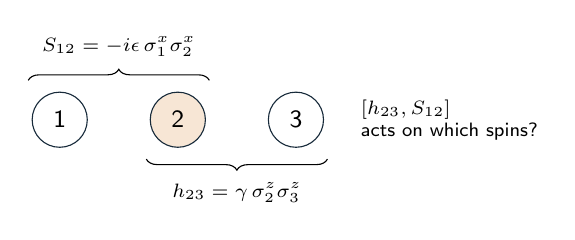
\begin{tikzpicture}[x=10mm,y=10mm,sp/.style={circle,draw=ink,minimum size=7mm,font=\small}]
\node[sp] (s1) at (0,0) {1};
\node[sp,fill=colA!20] (s2) at (1.5,0) {2};
\node[sp] (s3) at (3,0) {3};
\draw[decorate,decoration={brace,amplitude=4pt}] (-0.4,0.5)--(1.9,0.5) node[midway,above=5pt,font=\scriptsize]{$S_{12}=-i\epsilon\,\sigma^x_1\sigma^x_2$};
\draw[decorate,decoration={brace,amplitude=4pt,mirror}] (1.1,-0.5)--(3.4,-0.5) node[midway,below=5pt,font=\scriptsize]{$h_{23}=\gamma\,\sigma^z_2\sigma^z_3$};
\node[font=\scriptsize,anchor=west,align=left] at (3.7,0) {$[h_{23},S_{12}]$\\ acts on which spins?};
\end{tikzpicture}
\figtext{\textbf{Left (C.1).} The bare state $\ket0$ couples with strength $v$ to one excited state $\ket d$ that lies $\Delta$ higher. C.1 asks for the true lowest state of this $2\times2$ problem, and for the probability $P_d(t)$ of $\ket d$ if one starts in $\ket0$. Does the short-time growth of $P_d$ define a decay rate?
\textbf{Right (C.2).} A correction $S_{12}$ designed for spins 1--2 and a Hamiltonian term $h_{23}$ on spins 2--3 share spin 2 (orange). C.2 asks for their commutator and why it matters when corrections designed for separate pairs are put together along a chain.}
\end{figpanel}

\begin{redbox}{ADDED MODEL --- one double-excitation channel}
For C.1, retain only a bare two-cell reference $\ket{0}=\ket{o,o}$ (both particles in the reference orbital $o$) and one double excitation $\ket d$. A real cluster has many excited states; one denominator cannot replace that spectrum without a separate approximation.

\[
H_X=\begin{pmatrix}0&v\\v&\Delta\end{pmatrix},
\qquad v,\Delta>0,
\qquad\text{basis }(\ket0,\ket d).
\]
\end{redbox}
\question{C.1}{1.2}{Find the lower eigenvalue and a normalized lower eigenstate. Give their leading forms for $v/\Delta\ll1$. Starting from the bare state $\ket0$, find the exact double-excitation probability $P_d(t)$ and its short-time form. Does this probability define an irreversible decay rate?}

\begin{redbox}{ADDED MODEL --- an overlap diagnostic}
The following three-spin operators illustrate overlapping corrections on neighbouring clusters. They are illustrative and not fitted to any calculation:
\[
h_{23}=\gamma\,\sigma_2^z\sigma_3^z,\qquad
S_{12}=-i\epsilon\,\sigma_1^x\sigma_2^x,
\quad \gamma,\epsilon\in\mathbb R.
\]
\end{redbox}
\question{C.2}{0.6}{Calculate $[h_{23},S_{12}]$. Explain why a smaller residual on each isolated pair of cells does not, by itself, certify a small residual after the corrections are assembled along a chain.}
\origin{Use $[\sigma_z,\sigma_x]=2i\sigma_y$. Operators on different spins commute.}


\par\Needspace{14\baselineskip}\bigskip
\pagetitle{C.3. What survives the moving frame?}
\begin{greenbox}{GIVEN TOOL --- exact frame and source structure}
A number-conserving one-particle frame lifts to the complete many-body Fock space (T7). It does not delete modes or replace interactions by a mean field. A two-body interaction can still produce single and double excitations of a bare Slater reference.
\end{greenbox}
Let $W(t)$ be such a differentiable many-body frame. Set
\[
\mathcal K_W=W^\dagger H_{\rm MFP}W-iW^\dagger\dot W.
\]
For a differentiable anti-Hermitian many-body $S(t)$, let
\[
\mathcal U=We^S,\qquad
\ket{\zeta}=\mathcal U^\dagger\ket\Psi.
\]
Use the identity
\[
e^{-S}\partial_t e^S=\int_0^1e^{-uS}\dot S e^{uS}\,\dd u.
\]

\bridge{C.3}{1.2}{\textbf{(a)} Starting with $i\dot\Psi=H_{\rm MFP}\Psi$, derive the exact generator $\mathcal K_{\rm corr}$ of $\ket\zeta$ in terms of $\mathcal K_W,S,\dot S$.\par
\textbf{(b)} Identify the first-order terms if both $S$ and its time derivative belong to a controlled perturbative expansion. Why may $\dot S$ not simply be removed?\par
\textbf{(c)} If $\mathcal K_{\rm corr}=\mathcal K_{\rm ret}+\mathcal R$, where does an approximation first occur? Write the transformed physical initial state. Explain why dropping $\mathcal R$ needs a bound.\par
\textbf{(d)} Does the one-particle frame turn $H_{\rm int}$ into a one-particle operator? Does writing $e^S$ specify its coefficients or prove that it is local?}

\hint{For (b), expand $e^{-S}\mathcal K_We^{S}=\mathcal K_W+[\mathcal K_W,S]+\tfrac12[[\mathcal K_W,S],S]+\cdots$.}

\handoff{C.4 tests whether the kept part actually preserves the desired reference.}

\par\Needspace{14\baselineskip}\bigskip
\pagetitle{C.4. Does ``kept'' mean ``harmless''?}
\begin{greenbox}{GIVEN TOOL --- the kept generator}
This question asks what the kept part $\mathcal K_{\rm ret}$ of the generator does to a chosen reference state.
\end{greenbox}
For a fixed normalized direction $\ket{A_0}$ in the chosen frame, let $\Pi_A=\ket{A_0}\bra{A_0}$. Assume $\mathcal K_{\rm corr}=\mathcal K_{\rm ret}+\mathcal R$ as in C.3.

\bridge{C.4}{0.9}{\textbf{(a)} Give the necessary and sufficient instantaneous condition for $\mathcal K_{\rm ret}(t)$ to preserve $\ket{A_0}$ up to a phase throughout the interval.\par
\textbf{(b)} Return to the teaching spin chain of A.2, now with constant $g\ne0$. Take $\mathcal K_{\rm ret}=H_{\rm d}$ and $\mathcal R=0$. From the all-$A$ state, compute $(H_{\rm d}-E_A)\ket{A_0}$, its squared norm, and the leading short-time term of $\langle q_j(t)\rangle$, where $q_j=(1+\sigma_j^z)/2$.\par
\textbf{(c)} Has the retained model an approximation error in this example? Does zero omitted remainder prove that the reference direction is preserved? Does the short-time spin result give an MFP transport lifetime?}

\begin{redbox}{ADDED MODEL --- reuse A.2, do not infer an MB1 mapping}
The spin chain in (b) is still the teaching analogy, not the full MFP Hamiltonian. Use a ring of $N$ spins. Set $E_A=\bra{A_0}H_{\rm d}\ket{A_0}$. Let $\ket{j}$ denote the orthonormal configuration with only spin $j$ flipped. You may use $e^{-iHt}=\id-iHt+O(t^2)$.
\end{redbox}

\smallheading{A candidate reference evolution}
A candidate may have the form
\[
\ket{\Psi_{\rm ref}(t)}=W(t)e^{S(t)}\ket{\Xi(t)},\qquad
 i\dot\Xi=\mathcal K_{\rm ret}(t)\Xi.
\]

\begin{figpanel}{C.3 and C.4 --- changes of frame and what is kept}\label{fig:frames}
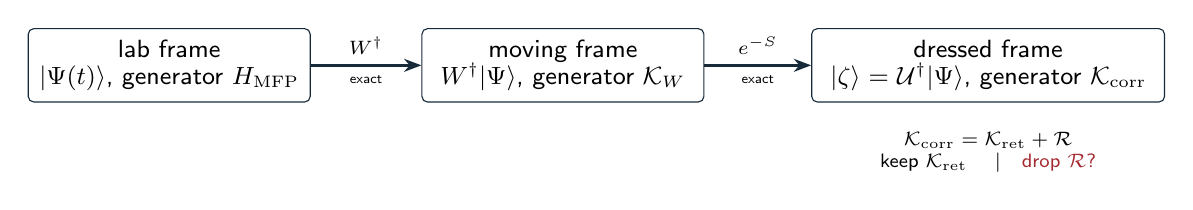
\begin{tikzpicture}[x=1mm,y=1mm]
\node[obj,text width=33mm] (L) at (0,0) {lab frame\\[-1pt]$\ket{\Psi(t)}$, generator $H_{\rm MFP}$};
\node[obj,text width=33mm] (M) at (50,0) {moving frame\\[-1pt]$W^\dagger\ket\Psi$, generator $\mathcal K_W$};
\node[obj,text width=42mm] (D) at (104,0) {dressed frame\\[-1pt]$\ket\zeta=\mathcal U^\dagger\ket\Psi$, generator $\mathcal K_{\rm corr}$};
\draw[okarrow] (L)--(M) node[midway,above,font=\scriptsize]{$W^\dagger$} node[midway,below,font=\tiny]{exact};
\draw[okarrow] (M)--(D) node[midway,above,font=\scriptsize]{$e^{-S}$} node[midway,below,font=\tiny]{exact};
\node[font=\scriptsize,align=center,below=2.5mm of D] {$\mathcal K_{\rm corr}=\mathcal K_{\rm ret}+\mathcal R$\\ keep $\mathcal K_{\rm ret}$ \quad\textbar\quad {\color{openred}drop $\mathcal R$?}};
\end{tikzpicture}

\medskip
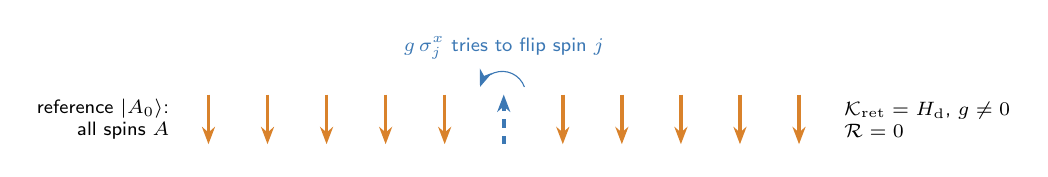
\begin{tikzpicture}[x=7.5mm,y=7.5mm]
\foreach \x in {0,...,10}{%
  \ifnum\x=5
    \draw[->,line width=1.3pt,colB,dashed] (\x,-0.42)--(\x,0.42);
  \else
    \draw[->,line width=1.3pt,colA] (\x,0.42)--(\x,-0.42);
  \fi}
\draw[->,colB] (5.35,0.55) arc (20:160:0.4);
\node[font=\scriptsize,text=colB,above] at (5,0.85) {$g\,\sigma^x_j$ tries to flip spin $j$};
\node[font=\scriptsize,anchor=east,align=right] at (-0.5,0) {reference $\ket{A_0}$:\\ all spins $A$};
\node[font=\scriptsize,anchor=west,align=left] at (10.6,0) {$\mathcal K_{\rm ret}=H_{\rm d}$, $g\neq0$\\ $\mathcal R=0$};
\end{tikzpicture}
\figtext{\textbf{Top (C.3).} Two exact changes of frame: first follow the geometry with $W$, then dress with correlations through $e^{S}$. C.3 asks for the exact generator in the dressed frame, and where the first approximation enters --- the only candidate is dropping the part $\mathcal R$.
\textbf{Bottom (C.4).} Suppose nothing is dropped ($\mathcal R=0$). C.4 asks whether the kept generator can still move the reference state $\ket{A_0}$. In the spin example the transverse field $g$ tries to flip each spin; part (b) asks how fast the flip probability of one spin starts to grow.}
\end{figpanel}

\nextpage
\parttitle{D}{The physical current}{2.0}
\begin{figpanel}{D.1 and D.2 --- current needs a phase; current through a twisted bond}\label{fig:current}
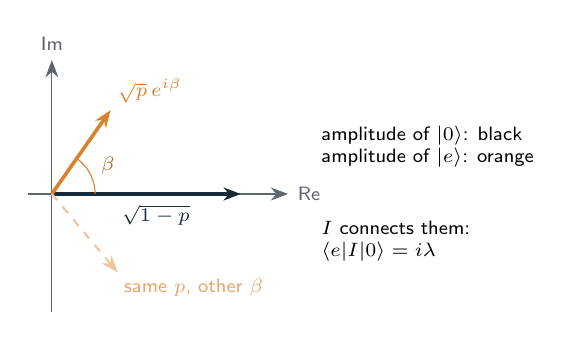
\begin{tikzpicture}[x=10mm,y=10mm]
\draw[->,rulegray] (-0.3,0)--(3.0,0) node[right,font=\scriptsize]{Re};
\draw[->,rulegray] (0,-1.5)--(0,1.7) node[above,font=\scriptsize]{Im};
\draw[->,line width=1.3pt,ink] (0,0)--(2.4,0) node[pos=0.55,below,font=\scriptsize]{$\sqrt{1-p}$};
\draw[->,line width=1.3pt,colA] (0,0)--(55:1.3) node[above right=-2pt,font=\scriptsize]{$\sqrt p\,e^{i\beta}$};
\draw[->,line width=0.8pt,colA!45,dashed] (0,0)--(-50:1.3) node[below right=-2pt,font=\scriptsize,text=colA!70]{same $p$, other $\beta$};
\draw[colA] (0.55,0) arc (0:55:0.55);
\node[font=\scriptsize,text=colA!80!black] at (27:0.8) {$\beta$};
\node[font=\scriptsize,align=left,anchor=west] at (3.3,0.6) {amplitude of $\ket0$: black\\ amplitude of $\ket e$: orange};
\node[font=\scriptsize,align=left,anchor=west] at (3.3,-0.6) {$I$ connects them:\\ $\bra eI\ket0=i\lambda$};
\end{tikzpicture}\hfill
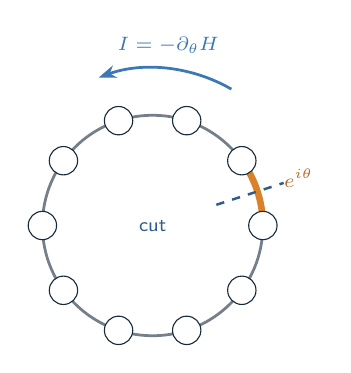
\begin{tikzpicture}[x=10mm,y=10mm]
\draw[ink!60,line width=1pt] (0,0) circle (1.4);
\draw[colA,line width=2.4pt] (0:1.4) arc (0:36:1.4);
\foreach \a in {0,36,...,324}{\node[site,minimum size=3.6mm] at (\a:1.4) {};}
\node[font=\scriptsize,text=colA!80!black] at (18:1.95) {$e^{i\theta}$};
\draw[dashed,figblue,line width=0.9pt] (18:0.85)--(18:1.75);
\draw[->,colB,line width=1pt] (60:2.0) arc (60:110:2.0);
\node[font=\scriptsize,text=colB] at (85:2.3) {$I=-\partial_\theta H$};
\node[font=\scriptsize,text=figblue,align=center] at (0,0) {cut};
\end{tikzpicture}
\figtext{\textbf{Left (D.1).} The probability $p$ fixes the lengths of the two amplitudes; the phase $\beta$ fixes their relative angle. D.1 asks how $\langle I\rangle$ depends on $\beta$ and, at small $p$, on $p$, and whether $p$ alone can fix the current.
\textbf{Right (D.2).} On a ring, put a phase $e^{i\theta}$ on one bond (a ``twist''). Then $I=-\partial_\theta H$ is the current through that bond. D.2 asks you to rewrite this same physical current after a change of frame $\mathcal U$, using $\mathcal K$ and $\mathcal A_\theta$, then to integrate it over time. The endpoint term $\langle\mathcal A_\theta\rangle$ is the piece one is tempted to drop.}
\end{figpanel}

\begin{redbox}{ADDED MODEL --- a current-connected pair of states}
For D.1, $\ket0$ and $\ket e$ are any orthogonal states connected by the stated current. Do not identify $\ket e$ with C.1's pure double excitation without checking the current matrix element. A one-body hopping current does not directly connect Slater determinants differing by two occupied orbitals.

\[
I=\lambda\begin{pmatrix}0&-i\\i&0\end{pmatrix},\qquad
\ket\psi=\sqrt{1-p}\ket0+e^{i\beta}\sqrt p\ket e,
\quad \lambda\in\mathbb R,\quad0\leq p\leq1.
\]
\end{redbox}
\question{D.1}{0.6}{Find $\langle I\rangle$ and compare $\beta=0,\pi/2,-\pi/2$. At small $p$, is the leading magnitude proportional to $p$ or to $\sqrt p$? Can the probability $p$ alone determine the current?}

\begin{greenbox}{GIVEN TOOL --- exact change of frame}
The current must be transformed with the same unitary as the Hamiltonian. Work on one smooth gauge patch and use the actual endpoint frame if a patch boundary is crossed. No approximation to the many-body state is made in D.2.

Introduce a boundary twist $\theta$: multiply the hopping on one chosen bond, from $j$ to $j+1$, by $e^{i\theta}$ (and its conjugate by $e^{-i\theta}$). Then $I=-\partial_\theta H$ at $\theta=0$ is the particle current through that bond. For a differentiable unitary $\mathcal U(\theta,t)$, define
\[
\mathcal A_\mu=i\mathcal U^\dagger\partial_\mu\mathcal U,
\qquad \mathcal K=\mathcal U^\dagger H\mathcal U-\mathcal A_t,
\qquad \mu\in\{\theta,t\}.
\]
You may use
\[
\partial_\theta\mathcal A_t-\partial_t\mathcal A_\theta
=i[\mathcal A_\theta,\mathcal A_t],
\]
and the rule T3 for time-dependent operators.
\end{greenbox}
\question{D.2}{1.4}{Prove that
$\mathcal U^\dagger I\mathcal U=-\partial_\theta \mathcal K-\partial_t\mathcal A_\theta-i[\mathcal K,\mathcal A_\theta]$.
For a state satisfying $i\partial_t\ket\Xi=\mathcal K\ket\Xi$, derive the integrated current from $t_1$ to $t_2$. Explain why a closed projector path does not justify deleting the endpoint term.}

\begin{redbox}{OPEN --- a current identity is not a current prediction}
The identity is exact. The full MFP problem still requires the driven correlated state, its physical current, and any endpoint or boundary contribution.
\end{redbox}


\nextpage
\parttitle{E}{Local accuracy in a large system}{2.4}

\begin{figpanel}{E.1--E.3 --- global overlap versus a local region}\label{fig:local}
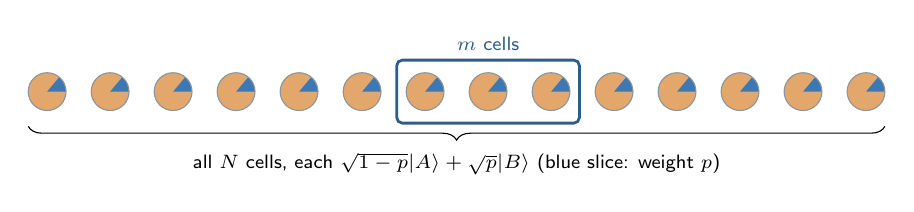
\begin{tikzpicture}[x=8mm,y=8mm]
\foreach \x in {0,...,13}{%
  \fill[colA!70] (\x,0) circle (0.3);
  \fill[colB] (\x,0)--++(0:0.3) arc (0:50:0.3)--cycle;
  \draw[ink!50] (\x,0) circle (0.3);}
\draw[figblue,rounded corners=2pt,line width=1pt] (5.55,-0.5) rectangle (8.45,0.5);
\node[font=\scriptsize,text=figblue,above] at (7,0.5) {$m$ cells};
\draw[decorate,decoration={brace,amplitude=5pt,mirror}] (-0.3,-0.55)--(13.3,-0.55) node[midway,below=6pt,font=\scriptsize]{all $N$ cells, each $\sqrt{1-p}\ket A+\sqrt p\ket B$ (blue slice: weight $p$)};
\end{tikzpicture}

\medskip
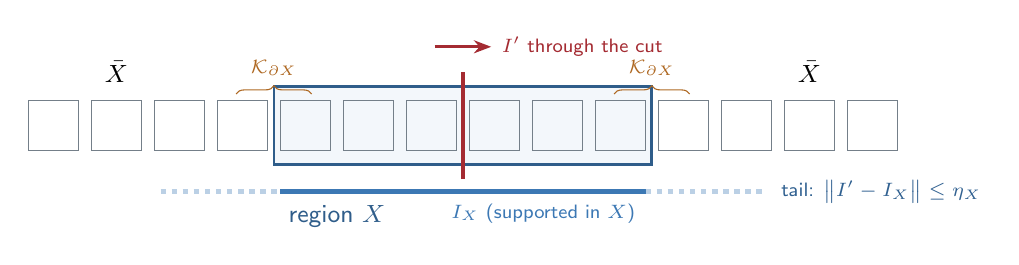
\begin{tikzpicture}[x=8mm,y=8mm]
\fill[figwash] (4,-0.62) rectangle (10,0.62);
\foreach \x in {0,...,13}{\draw[ink!60] (\x+0.1,-0.4) rectangle (\x+0.9,0.4);}
\draw[figblue,line width=1pt] (4,-0.62) rectangle (10,0.62);
\node[font=\small,text=figblue] at (5.0,-1.45) {region $X$};
\node[font=\small] at (1.5,0.85) {$\bar X$};
\node[font=\small] at (12.5,0.85) {$\bar X$};
\draw[openred,line width=1.4pt] (7,-0.85)--(7,0.85);
\draw[->,openred,line width=1pt] (6.55,1.25)--(7.45,1.25) node[right,font=\scriptsize]{$I'$ through the cut};
\draw[decorate,decoration={brace,amplitude=3pt},colA!80!black] (3.4,0.5)--(4.6,0.5) node[midway,above=3pt,font=\scriptsize]{$\mathcal K_{\partial X}$};
\draw[decorate,decoration={brace,amplitude=3pt},colA!80!black] (9.4,0.5)--(10.6,0.5) node[midway,above=3pt,font=\scriptsize]{$\mathcal K_{\partial X}$};
\draw[line width=2pt,colB] (4.1,-1.05)--(9.9,-1.05) node[pos=0.72,below,font=\scriptsize]{$I_X$ (supported in $X$)};
\draw[line width=2pt,colB!35,dotted] (2.2,-1.05)--(4.1,-1.05);
\draw[line width=2pt,colB!35,dotted] (9.9,-1.05)--(11.8,-1.05);
\node[font=\scriptsize,text=colB!80!black,anchor=west] at (11.9,-1.05) {tail: $\norm{I'-I_X}\le\eta_X$};
\end{tikzpicture}
\figtext{\textbf{Top (E.1).} Every cell is slightly imperfect. E.1 compares the overlap with the ideal all-$A$ state for the whole chain and for a fixed window of $m$ cells, and asks what this says about global fidelity as a test of local transport.
\textbf{Bottom (E.2, E.3).} The current is measured at the red cut. E.2 asks you to replace $I'$ by an operator $I_X$ supported in a region $X$ around the cut, and to bound the current error by the distance between the two states reduced to $X$, plus the small tail $\eta_X$. E.3 asks which equation the reduced state $\sigma'_X$ obeys; the terms $\mathcal K_{\partial X}$ that cross the edge of $X$ are the reason the outside matters.}
\end{figpanel}

\begin{redbox}{ADDED STATE --- a diagnostic product family}
For E.1 only, prescribe the state below. It is not asserted to be a solution of the interacting pump. The scalar $p$ is independent of $N$. Use the squared-fidelity convention $\mathcal F(\rho,\ket a)=\bra a\rho\ket a$.

\[
\ket{\psi_N}=\bigotimes_{j=1}^N
\big[\sqrt{1-p}\ket A_j+\sqrt p\ket B_j\big],
\qquad0<p<1,\quad\braket A B=0.
\]
\end{redbox}
\question{E.1}{0.5}{Find its fidelity with $\ket A^{\otimes N}$. Then find the fidelity of an $m$-cell subsystem with $\ket A^{\otimes m}$, with $m$ fixed as $N$ increases. What does this comparison imply about using global fidelity to diagnose local transport?}

\begin{greenbox}{GIVEN TOOL --- local current-error structure}
In E.2, use a local observable and reduced states rather than global many-body overlap. The inequality can be derived without a small-error or weak-interaction assumption.
\end{greenbox}

Let $\rho'$ and $\sigma'$ be normalized density matrices in the same moving frame: $\rho'$ is the exact transformed state and $\sigma'$ the reference. Let $I_X$ be supported near the measured cut, in a region $X$, and suppose $\norm{I'-I_X}\leq\eta_X$. Reduced density matrices on $X$ are denoted by $\rho'_X$ and $\sigma'_X$ (T6). Set $\Delta I=\Tr[(\rho'-\sigma')I']$.

\question{E.2}{1.0}{Prove
$|\Delta I|\leq\norm{I_X}\norm{\rho'_X-\sigma'_X}_1+2\eta_X$.
If the reference is a product state in this frame, define
$q_x=1-\ket{A_{0,x}}\bra{A_{0,x}}$ and
$D_X=\sum_{x\in X}\langle q_x\rangle_{\rho'}$.
Deduce
$|\Delta I|\leq2\norm{I_X}\min(1,\sqrt{D_X})+2\eta_X$.
State which form remains valid for a general correlated reference.}

\smallheading{Useful facts}
\[
\begin{gathered}
|\Tr(AB)|\leq\norm A_1\norm B,\qquad
\norm{\rho-\sigma}_1\leq2,\\
\norm{\rho-\ket a\bra a}_1\leq
2\sqrt{1-\bra a\rho\ket a},\\
1-\prod_{x\in X}(1-q_x)\leq\sum_{x\in X}q_x.
\end{gathered}
\]
\origin{Here $\norm{\cdot}$ is the operator norm and $\norm{\cdot}_1$ is the trace norm. The local $q_x$ are reference-deviation operators, not automatically physical domain counters.}

\par\Needspace{14\baselineskip}\bigskip
\pagetitle{E.3. From a kept Hamiltonian to a local state}
\begin{greenbox}{GIVEN TOOL --- same physical current, local states}
The current-error inequality of E.2 uses two local reduced states in the same frame. It does not supply their dynamics. This question makes that missing input explicit, without introducing a heat bath.
\end{greenbox}
Let the exact transformed state be $\rho'$ and the reference state be $\sigma'$. Suppose
\[
\begin{split}
i\dot\rho'&=[\mathcal K_{\rm corr},\rho'],\\
i\dot\sigma'&=[\mathcal K_{\rm ret},\sigma'],\\
\mathcal K_{\rm corr}&=\mathcal K_{\rm ret}+\mathcal R.
\end{split}
\]
Both states are normalized. Their initial values must be stated; they need not coincide. For a region $X$ near a cut, write
\[
\mathcal K_{\rm ret}=\mathcal K_X+\mathcal K_{\bar X}+\mathcal K_{\partial X},\qquad
\sigma'_X=\Tr_{\bar X}\sigma'.
\]
The first two terms act only inside and outside $X$. The third contains interactions that connect both regions.

\bridge{E.3}{0.9}{\textbf{(a)} Derive the equation for $\sigma'_X$. Show why the contribution from $\mathcal K_{\bar X}$ vanishes under the partial trace.\par
\textbf{(b)} Is $\sigma'_X(0)$ and $\mathcal K_X(t)$ enough to solve that equation? Identify the additional object required by the boundary term. Does the composite-band gap supply it?\par
\textbf{(c)} Let $\delta\rho=\rho'-\sigma'$. Derive its exact equation and identify the initial-mismatch and omitted-dynamics inputs. Explain why rewriting this equation is not yet a bound on $\norm{\delta\rho_X(t)}_1$.}

\smallheading{Useful fact}
For an operator $B_{\bar X}$ supported outside $X$, the partial trace is cyclic with respect to that operator:
\[
\Tr_{\bar X}(B_{\bar X}A)=\Tr_{\bar X}(AB_{\bar X}).
\]
\handoff{D.2 supplies the correct current operator. E.2 converts a local-state error into a current error. E.3 identifies the missing dynamics between these two tools.}

\nextpage
\parttitle{F}{A conditional operating-time certificate}{1.5}
\begin{redbox}{GIVEN BOUNDS --- the missing long-time inputs}
Let $\alpha,I_0>0$ and $\eta,\delta_0\geq0$. Assume that, for every $0\leq s\leq t_{\max}$,
\[
D_X(s)\leq\alpha^2s^2,\qquad
\norm{I_X(s)}\leq I_0,\qquad\eta_X(s)\leq\eta.
\]
Also assume that every relevant two-period reference window satisfies
$|\Qbar_{\rm ref}(t)-Q_*|\leq\delta_0$.
These remain supplied assumptions for the full correlated MB1 frame. In particular, the bound at $s=0$ requires $D_X(0)=0$. Initial mismatch must be controlled separately; do not silently replace the physical initial state by its projection. Here $\alpha$, $I_0$, and $\eta$ have units of inverse time; $\delta_0$ and charge are dimensionless.
\end{redbox}

Define
\[
\Qbar(t)=\frac12\int_{t-2T}^{t}\langle I(s)\rangle\,\dd s,
\qquad2T\leq t\leq t_{\max},
\]
and $\Qbar_{\rm ref}(t)$ in the same way with the reference state. The factor is $1/2$, not $1/(2T)$: this is charge per drive period averaged over two periods, not mean current.

\question{F.1}{0.7}{Use E.2 to bound $|\Qbar(t)-Q_*|$. For $\alpha I_0>0$, find a sufficient upper endpoint $t_{\rm cert}$ for which this bound is at most a tolerance $\delta$. State the positivity and time-domain conditions. Evaluate the result with the illustrative inputs below. Does the next period necessarily fail?}

\begin{redbox}{ILLUSTRATIVE NUMBERS --- not MB1 measurements}
Use the time unit $\tau_0=T$, so $T/\tau_0=1$. Let
\[
I_0\tau_0=1,\quad\alpha\tau_0=10^{-5},\quad
\eta\tau_0=10^{-5},\quad
\delta_0=0.001,\quad\delta=0.005.
\]
Assume $t_{\max}=201\tau_0$. These numbers are chosen for arithmetic practice. They must not be quoted as an MFP lifetime result.
\end{redbox}

\smallheading{Connection to C.4}
The product-reference form of E.2 compares $\rho'$ with the \emph{fixed} direction $\ket{A_{0,X}}$. It is therefore the right tool only while the reference state itself stays on that direction --- exactly the property tested in C.4(a). C.4(b) showed that kept dynamics can move the reference even when $\mathcal R=0$. In that case the premise $D_X(s)\le\alpha^2s^2$ for a fixed product reference is not the right input; one must use the general form of E.2 with an evolving reference, as in F.3.

\begin{figpanel}{F.1 --- a sliding two-period window}\label{fig:window}
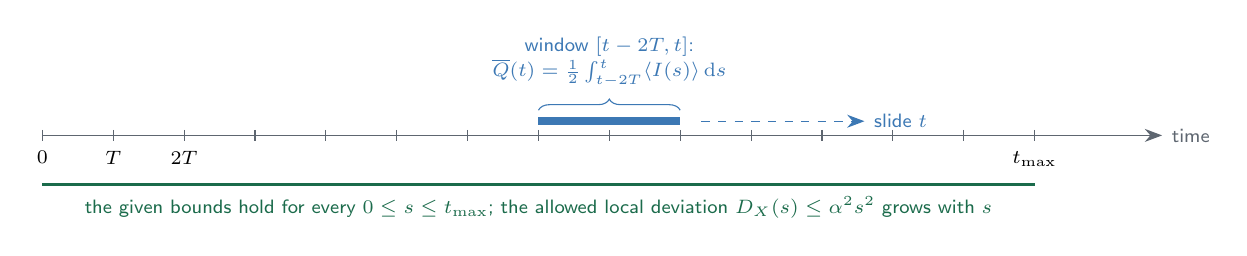
\begin{tikzpicture}[x=9mm,y=10mm]
\draw[->,rulegray] (0,0)--(15.8,0) node[right,font=\scriptsize]{time};
\foreach \n in {0,...,14}{\draw[rulegray] (\n,0.07)--(\n,-0.07);}
\node[font=\scriptsize,below] at (0,-0.08) {$0$};
\node[font=\scriptsize,below] at (1,-0.08) {$T$};
\node[font=\scriptsize,below] at (2,-0.08) {$2T$};
\node[font=\scriptsize,below] at (14,-0.08) {$t_{\max}$};
\draw[sourcegreen,line width=1.2pt] (0,-0.62)--(14,-0.62);
\node[font=\scriptsize,text=sourcegreen,below] at (7,-0.65) {the given bounds hold for every $0\le s\le t_{\max}$; the allowed local deviation $D_X(s)\le\alpha^2s^2$ grows with $s$};
\draw[colB,line width=3pt] (7,0.18)--(9,0.18);
\draw[decorate,decoration={brace,amplitude=4pt},colB] (7,0.32)--(9,0.32) node[midway,above=5pt,font=\scriptsize,align=center]{window $[t-2T,t]$:\\ $\Qbar(t)=\frac12\int_{t-2T}^{t}\langle I(s)\rangle\,\dd s$};
\draw[->,dashed,colB] (9.3,0.18)--(11.6,0.18) node[right,font=\scriptsize]{slide $t$};
\end{tikzpicture}
\figtext{Every window of length $2T$ gives one averaged charge $\Qbar(t)$. The given bounds allow the local deviation from the reference to grow with time. \textbf{F.1 asks:} up to which window end $t$ can you still guarantee $|\Qbar(t)-Q_*|\le\delta$, and what can be said about the windows after that time?}
\end{figpanel}

\par\Needspace{14\baselineskip}\bigskip
\pagetitle{F.3. Prediction, error, and first failure}
\begin{greenbox}{GIVEN TOOL --- the observable inequality}
For the same frame and the same physical current, E.2 gives
\[
|\Delta I(s)|\leq\norm{I_X(s)}\norm{\rho'_X(s)-\sigma'_X(s)}_1+2\eta_X(s).
\]
A reference charge must be calculated from its state. It is not assigned the target $Q_*$ solely from a geometric winding.
\end{greenbox}
Define $\widehat Q(t)=\tfrac12\int_{t-2T}^{t}\Tr[\sigma'(s)I'(s)]\,\dd s$. For this exercise, suppose computable functions satisfy
\[
\norm{\rho'_X(s)-\sigma'_X(s)}_1\leq e_X(s),\qquad
\norm{I_X(s)}\leq b_X(s),\qquad
\eta_X(s)\leq\eta(s).
\]

\bridge{F.3}{0.8}{\textbf{(a)} Integrate the current inequality to obtain $|\Qbar(t)-\widehat Q(t)|\leq E(t)$. State where initial mismatch must enter this construction.\par
\textbf{(b)} Derive sufficient tests to certify that a given window is inside or outside the tolerance $|\Qbar-Q_*|\leq\delta$. What is the output when neither test holds?\par
\textbf{(c)} Apply the tests to the three supplied sample windows. Is the first failed sampled window determined? Is the first failure over continuously varying window starts determined?}

\begin{redbox}{GIVEN FUNCTIONS AND NUMBERS --- teaching inputs only}
The functions above are not established MB1 bounds. For the arithmetic test take $Q_*=-0.5$ and $\delta=0.005$:
\begin{center}\begin{tabular}{@{}lrr@{}}\toprule
Ordered sample window&$\widehat Q$&$E$\\\midrule
1&$-0.4970$&$0.0010$\\
2&$-0.4940$&$0.0015$\\
3&$-0.4940$&$0.0005$\\\bottomrule
\end{tabular}\end{center}
These are invented classification examples, not new trajectories. Use one-window exceedance; no persistence rule is imposed in this small exercise.
\end{redbox}

\begin{figpanel}{F.3 --- a prediction with an error bar}\label{fig:interval}
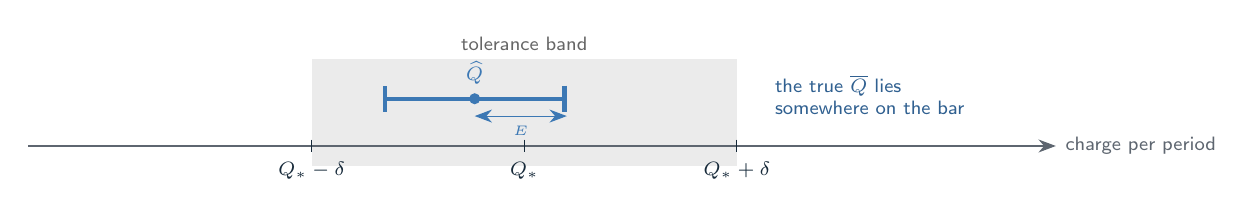
\begin{tikzpicture}[x=9mm,y=10mm]
\fill[black!8] (4,-0.25) rectangle (10,1.1);
\draw[->,rulegray] (0,0)--(14.5,0) node[right,font=\scriptsize]{charge per period};
\draw[ink] (7,0.08)--(7,-0.08) node[below,font=\scriptsize]{$Q_*$};
\draw[ink] (4,0.08)--(4,-0.08) node[below,font=\scriptsize]{$Q_*-\delta$};
\draw[ink] (10,0.08)--(10,-0.08) node[below,font=\scriptsize]{$Q_*+\delta$};
\node[font=\scriptsize,text=black!60] at (7,1.3) {tolerance band};
\draw[colB,line width=1.6pt,|-|] (5.0,0.6)--(7.6,0.6);
\fill[colB] (6.3,0.6) circle (2pt);
\node[font=\scriptsize,text=colB,above] at (6.3,0.66) {$\widehat Q$};
\draw[<->,colB] (6.3,0.38)--(7.6,0.38) node[midway,below,font=\tiny]{$E$};
\node[font=\scriptsize,text=colB!80!black,anchor=west,align=left] at (10.4,0.65) {the true $\Qbar$ lies\\ somewhere on the bar};
\end{tikzpicture}
\figtext{A computed prediction $\widehat Q$ for one window, with a proven error $E$: the true $\Qbar$ lies on the blue bar. \textbf{F.3 asks:} for which positions of the bar relative to the grey band can you certify ``inside'', certify ``outside'', or neither? Then apply your rule to three given windows.}
\end{figpanel}

\handoff{F.1 certifies an interval once special growth bounds are supplied. F.3 permits a reference that itself changes or fails. Both require model-derived inputs before either gives an MB1 prediction.}

\nextpage
\parttitle{X}{Synthesis: what would a prediction need?}{0.5}
\begin{greenbox}{SUMMARY --- the tools now on the table}
The sources supply the candidate flavor mechanism [1] and projector kinematics [2]. This booklet adds exact frame, current and local-error identities. A full correlated pump is still missing.
\end{greenbox}
\begin{redbox}{OPEN --- the research task}
Starting from $H_{\rm MFP}(t)$ and a specified physical initial state, construct a correlated reference evolution and a computable error estimate over complete drive cycles. The result must remain useful as the system size increases. Do not import F.1's long-time assumptions as facts.
\end{redbox}

Seek a prediction $\widehat Q(t)$ and an error $E(t)$ such that
\[
|\Qbar(t)-\widehat Q(t)|\leq E(t),
\]
and the two tests
\[
\begin{array}{ll}
|\widehat Q-Q_*|+E\leq0.005
&\text{certifies that the window passes},\\[3pt]
|\widehat Q-Q_*|-E>0.005
&\text{certifies that the window fails}.
\end{array}
\]

\question{X.1}{0.5}{List the inputs that must be derived from $H_{\rm MFP}$ and a specified physical initial state before either test can be applied to the original pump. Why does certifying individual windows not, by itself, locate the first failure?}

\smallheading{What a correct answer does not prove}
A solved toy model does not establish its equivalence to MFP. A checked matrix identity does not establish a small full-chain remainder. A certified lower bound is not an exact lifetime. These distinctions are part of the problem.

\nextpage
\pagetitle{Sources}
\sourceentries

\smallheading{Optional background reading (public; not needed for any question)}
{\small\begin{itemize}[leftmargin=6mm,itemsep=2pt,topsep=2pt]
\item Thouless pumps: R.~Citro and M.~Aidelsburger, \emph{Thouless pumping and topology}, Nat.\ Rev.\ Phys.\ \textbf{5}, 87 (2023), \href{https://arxiv.org/abs/2210.02050}{\texttt{arXiv:2210.02050}}.
\item Berry phase and adiabatic transport: D.~Xiao, M.-C.~Chang, and Q.~Niu, Rev.\ Mod.\ Phys.\ \textbf{82}, 1959 (2010), \href{https://arxiv.org/abs/0907.2021}{\texttt{arXiv:0907.2021}}.
\item Wannier functions and Wilson loops: N.~Marzari \emph{et al.}, Rev.\ Mod.\ Phys.\ \textbf{84}, 1419 (2012), \href{https://arxiv.org/abs/1112.5411}{\texttt{arXiv:1112.5411}}.
\item Exponential localization: C.~Brouder \emph{et al.}, PRL \textbf{98}, 046402 (2007), \href{https://arxiv.org/abs/cond-mat/0606726}{\texttt{arXiv:cond-mat/0606726}}.
\item Dressing transformations $e^S$: S.~Bravyi, D.~P.~DiVincenzo, and D.~Loss, Ann.\ Phys.\ \textbf{326}, 2793 (2011), \href{https://arxiv.org/abs/1105.0675}{\texttt{arXiv:1105.0675}}.
\item Domain formation in spin chains: G.~Lagnese \emph{et al.}, Phys.\ Rev.\ B \textbf{104}, L201106 (2021), \href{https://arxiv.org/abs/2107.10176}{\texttt{arXiv:2107.10176}}.
\item Trace distance and fidelity: C.~A.~Fuchs and J.~van de Graaf, \href{https://arxiv.org/abs/quant-ph/9712042}{\texttt{arXiv:quant-ph/9712042}}.
\item Position operator on a ring (used for Pictures~\ref{fig:conveyor}): R.~Resta, Phys.\ Rev.\ Lett.\ \textbf{80}, 1800 (1998).
\end{itemize}}

\begin{redbox}{The main scientific gap}
Neither source supplies a controlled full-cycle correlated reference, its physical current, or a quantitative large-system lifetime. Red frames mark those missing links.
\end{redbox}

The solution booklet contains worked answers and marking notes.
\vfill
\begin{center}\textbf{End of question booklet}\end{center}
\end{document}
